% !TeX encoding = UTF-8
% !TeX TS-program = pdflatex
% !TeX spellcheck = de_DE

\def\version{\today L. Schink)}
% Verlauf
% v 1.1 20.2.20202 S. Schramm - Initiale Version
% v 1.2 20.2.20202 A. Dürrbaum - Anpassungen Ttielseite / Indices

% Dokumenteneinstellung
\documentclass[a4paper,11pt,cleardoubleempty]{scrbook}

%% Einstellungsdatei
% !TeX spellcheck = de_DE

% Do's & Dont's in LaTeX
%\RequirePackage[l2tabu,orthodox]{nag}

% Deutsch und UTF-8 Encoding
\usepackage[english,ngerman]{babel}
\selectlanguage{ngerman}

\usepackage[utf8]{inputenc}
\usepackage[T1]{fontenc}
\usepackage{lmodern}

% Seiteneinstellungen
\usepackage{geometry}
\geometry{left=35mm,right=35mm, bindingoffset=0mm, top=30mm,bottom=30mm}

% Abstand im Text
\usepackage{xspace}
\usepackage{setspace}

% Kapitelüberschrift: große Nummer -> Titel
\renewcommand*{\chapterformat}{\mbox{\chapappifchapterprefix{\nobreakspace}\scalebox{3}{\thechapter}\enskip}}

% Linie unter \chapter
\makeatletter
\renewcommand{\chapterlinesformat}[3]{%
  \parbox[t]{\linewidth}{%
    \raggedchapter\@hangfrom{#2}{#3}\par%
    \vspace*{-.75\ht\strutbox}\rule{\linewidth}{.8pt}%
  }%
}
\makeatother

% pdf Pakete
\usepackage[pdfusetitle=true,colorlinks=true,linkcolor=blue,urlcolor=blue,citecolor=blue,bookmarks=true,bookmarksopenlevel=2]{hyperref}

% Pakete für Grafiken
\usepackage{graphicx}
\usepackage{color}
\usepackage{xcolor}
\usepackage{tikz}
\usepackage{pgfplots}
\pgfplotsset{compat=1.5}
\usepackage{caption}
\captionsetup{labelfont=bf, textfont=small} 
\usepackage{subcaption}

% Tabellentools
\usepackage{tabularx}
\usepackage{supertabular}
\usepackage{multirow}
\usepackage{multicol}

% Mathematik
\usepackage[fleqn]{amsmath}
\usepackage{amssymb,amsthm,textcomp}
\usepackage{upgreek}

% Zahlenformate
\usepackage{siunitx}
\sisetup{range-phrase=\ \textrm{bis}\ }
\sisetup{locale=DE}

% Auflistungen
\usepackage{enumerate}

% Symbolverzeichnis
\usepackage[nomentbl]{Einstellungen/nomencl-table}

% Glossar
%\usepackage[nonumberlist,toc,nopostdot,style=alttree,xindy]{glossaries}
\usepackage{glossaries}

% Index
\usepackage{makeidx}

% Listings
\usepackage{listings}

% Eigene Tabellenspalten
\usepackage{tabularx}
\usepackage{dcolumn}

%%%%%%%%%%%%%%%%%%%%%%%%%%%%%%%%%%%%%%%%%%%%%%%%%%%%%%%%%%%%%%%%%%%%%%%%%%%%%%
% HIER EIGENE PAKETE HINZUFÜGEN
%
%
%
%
%%%%%%%%%%%%%%%%%%%%%%%%%%%%%%%%%%%%%%%%%%%%%%%%%%%%%%%%%%%%%%%%%%%%%%%%%%%%%%
% Vor dem Laden von weiteren Paketen in das Latex-Sündenregister von Marc Ensenbach schauen!
%%%%%%%%%%%%%%%%%%%%%%%%%%%%%%%%%%%%%%%%%%%%%%%%%%%%%%%%%%%%%%%%%%%%%%%%%%%%%%

%%%%% Sonstiges

% Es können todo-Notes eingefügt werden
\usepackage{todonotes}

% Definition der Kopf und Fußzeilen
\usepackage{fancyhdr,lastpage}
\fancypagestyle{fancy2}{%
	\fancyhf{}
	\fancyhead[L]{}
	\fancyhead[C]{}
	\fancyhead[R]{}
	\fancyfoot[OL]{}
	\fancyfoot[EL]{\thepage}
	\fancyfoot[C]{ }
	\fancyfoot[OR]{\thepage}
	\fancyfoot[ER]{}
	\renewcommand{\headrulewidth}{1pt}
	\renewcommand{\footrulewidth}{1pt}
}
\fancypagestyle{plain}{%
	\fancyhf{}%
	\renewcommand{\headrulewidth}{0pt}%
	\renewcommand{\footrulewidth}{0pt}
	\fancyfoot[OR]{\thepage}
}
\renewcommand{\headrulewidth}{0pt}
\renewcommand{\footrulewidth}{0pt}
\usepackage{emptypage}

% \matr{A} ergibt "fettes A" wie es bei Matrizen aussehen soll
\newcommand{\matr}[1]{\mathbf{#1}}

% Definition der Uni Kassel Farbpalette
\definecolor{UKDunkelGrau}{RGB}{87,87,87}
\definecolor{UKMittelGrau}{RGB}{157,157,157}
\definecolor{UKHellGrau}{RGB}{218,218,218}
\definecolor{UKDunkelPink}{RGB}{154,12,70}
\definecolor{UKMittelPink}{RGB}{199,16,92}
\definecolor{UKHellPink}{RGB}{243,216,221}
\definecolor{UKGruen}{RGB}{21,56,36}
\definecolor{UKBlau}{RGB}{80,149,200}
\definecolor{UKGelb}{RGB}{196,210,15}
\definecolor{UKTuerkis}{RGB}{74,172,150}
\definecolor{UKGold}{RGB}{234,195,114}

%%%%%%%%%%%%%%%%%%%%%%%%%%%%%%

\renewcommand{\familydefault}{\rmdefault}
\renewcommand*\rmdefault{ppl}

\setlength{\parindent}{0pt}
\setlength{\parskip}{6pt}

\makeatletter
% !TeX spellcheck = de_DE
\renewcommand{\maketitle}{\fontfamily{cmss}\selectfont
  \begin{center}
	\vspace*{-0.5cm}
	\includegraphics[width=75mm]{Bilder/UniKS-Logo}\\

	\vspace{1.5cm}
	\centering
        \ifthenelse{\equal{\Typ}{MSc}}{
	% Masterarbeit
	\textbf{\Large Masterarbeit}\\[1ex]
        }{\ifthenelse{\equal{\Typ}{BSc}}{
	% Bachelorarbeit
	\textbf{\Large Bachelorarbeit}\\[1ex]
        }{
        %  Restliche Arbeiten:
	\textbf{\Large \Typ}\\[4ex]
        }}
	\textsf{\Huge \@title}\\[4ex]
%
	{\Large \@author}\\[4ex]
%
        \ifthenelse{\isundefined{\Titelgrafik}}{}{
  	  \vfill
          \includegraphics[height=8cm]{\Titelgrafik}
  	  \vfill
        }
	\vfill
        \ifthenelse{\equal{\Typ}{Technischer Bericht}}{
        Bericht-Nr. \MRTnr\\  
        }{ 
        \begin{center}
          %\fbox{\parbox{14cm}{
          \renewcommand{\arraystretch}{1.2}
		\begin{tabularx}{\columnwidth}{p{0.5\textwidth}>{\raggedleft\arraybackslash}p{0.5\textwidth}}
			Matrikelnummer: & \MatNr\\
                        \ifthenelse{\equal{\Typ}{MSc}\or\equal{\Typ}{BSc}}{
			Erstgutachter: & \Erstgutachter\\
			Zweitgutachter: & \Zweitgutachter\\}{
			Gutachter: & \Erstgutachter\\}
                        \ifthenelse{\isundefined{\Betreuer}}{}{
			Betreuer: & \Betreuer\\}
			Tag der Abgabe: & \@date\\
                        \ifthenelse{\isundefined{\MRTnr}}{}{MRT-Nr.:& \MRTnr\\}
                      \end{tabularx}%
            %          }}
                    \end{center}
        }
	\vfill
	\includegraphics[height=12mm]{Bilder/MRT-Logo} \hfill \includegraphics[height=12mm]{Bilder/ISAC-Logo}
\end{center}
}


%%% Local Variables:
%%% mode: latex
%%% TeX-master: "../MRT-Bericht-2020"
%%% End:

\makeatother

\newcounter{SeitenzahlSpeicher}

%%% Local Variables:
%%% mode: latex
%%% TeX-master: "../MRT-Bericht-2020"
%%% End:


%% Alternative zu Schriftart Calibri
\usepackage[sfdefault,lf]{carlito}


%% Benötigte Daten!
\title{\fontsize{16}{14}\selectfont Von C\# nach Python: Software-Konzeptionierung einer robotergestützten Lagerverwaltung\\
{\fontsize{10}{10}\selectfont Analyse bestehender Software und Konzeptionierung einer integrierten Python-Anwendung mit kameragestützen Validierungsprozessen in der Industrie 4.0-Plattform Modellfabrik $\mu$Plant}}
\date{\today}
\author{Lennart Schink}
\def\MatNr{33237484}
 
%% Wenn \geburtsort auskommentiert -> Ausgabe von
%%  Geburtsag und Geburtsort auf Deckblatt
\def\Geburtsort{Bad Bergzabern}\def\Geburtstag{31.12.1990}

%% Art des Berichtes (eines auskommentieren)
%\def\Typ{MSc}
\def\Typ{Seminararbeit}
%\def\Typ{BSc}
%\def\Typ{Seminararbeit}
%\def\Typ{Technischer Bericht}

%% MRT-Nummer, wenn schon bekannt
\def\MRTnr{N.N}

%% Auskommentieren, wenn eine Grafig auf dem Titelblatt erscheinen sollen
% maximale Höhe: 5cm, max. Breite 15 cm
%\def\Titelgrafik{Bilder/Wissenschaft.jpg}

%% Gutachter
\def\Erstgutachter{Univ.-Prof.~Dr.-Ing. Andreas Kroll}
%\def\Zweitgutachter{Dr.-Ing. Robert Schmoll } % nur bei MSc oder BSc

%% Auskommentieren, wenn der/die Betreuer auf dem Titelblatt erscheinen sollen
\def\Betreuer{Dip.-Ing. Axel Dürrbaum} % Mehrer Betreuer möglich

%% PDF mit Aufgabenstellung
\def\Aufgabenstellung{Bilder/Aufgabenstellung.pdf}

%% MRT-Informationen im PDF
\pdfinfo{
   /Author \@author
   /Title \@title
   /CreationDate \@date
   /Subject \Typ
   /Keywords (MRT;LaTeX)
}


% --------------------------------------------------------------------
% Benutzerdefinierte Makros
% --------------------------------------------------------------------

% Schreibweise für Vektoren
\def\Vektor#1{\ensuremath{\mathbf{#1}}}

% Transponieren einesVektors/einer Matrix
\def\Trans#1{\ensuremath{#1^{\mathrm{T}}}}

% Variable/Zahlenwert mit Einheit
\def\Einheit#1#2{\ensuremath{#1 \text{ in } \mathrm{#2}}}

% --------------------------------------------------------------------
% Abkürzungsverzeichnis
\makeglossary
\newcommand*{\Glossar}[3]{#3 (\gls{#1})\newglossaryentry{#1}{name=#2,
    description={#3}}}

% Symbolverzeichnis
\makenomenclature
\renewcommand{\nomname}{Symbolverzeichnis}
\newcommand*{\Symbol}[2]{#1\nomenclature{#1}{#2}{}{}}
\newcommand*{\SymbolT}[2]{#2 #1\nomenclature{#1}{#2}{}{}}
\newcommand*{\SymbolE}[3]{#2 #1\nomenclature{#1}{#2}{#3}{}}
\newcommand*{\SymbolB}[4]{#2 #1\nomenclature{#1}{#2}{#3}{#4}}

% Index
\makeindex
\newcommand*{\Index}[1]{#1\index{#1}}

% --------------------------------------------------------------------
  
% Beginn des Dokuments
\begin{document}
\pagenumbering{Roman}

% Bei Problemen mit überhängenden Absätzen kann Sloppy zur Aufweichung
% der Satzparameter genutzt werden. Dies wird offiziell nicht
% empfohlen, kann aber u. U. zu guten Ergebnissen führen.
%\sloppy

% --------------------------------------------------------------------------
% Titelseite (IMMER)
% --------------------------------------------------------------------------
\fancyhf{}
\pagestyle{empty}
\maketitle 
\cleardoublepage

% --------------------------------------------------------------------------
% Aufgabenstellung (IMMER) 
% PDF-Aufgabenstellung von Betreuer geben lassen und hier einfügen
% --------------------------------------------------------------------------
\ifthenelse{\equal{\Typ}{MSc}\or\equal{\Typ}{BSc}}{
\begin{figure}[!htbp]\centering
\fbox{\includegraphics[width=1.0\textwidth,page=1]{\Aufgabenstellung}}
\end{figure}

\begin{figure}[!htbp]
\centering
\fbox{\includegraphics[width=1.0\textwidth,page=2]{\Aufgabenstellung}}
\end{figure}
\cleardoublepage
}{}

% --------------------------------------------------------------------------
% Versicherung (BEI BA UND MA)
% --------------------------------------------------------------------------
\ifthenelse{\equal{\Typ}{MSc}\or\equal{\Typ}{BSc}}{
% !TeX encoding = UTF-8
% !TeX TS-program = pdflatex
% !TeX spellcheck = de_DE

\chapter*{Versicherung}

Hiermit versichere ich, dass ich die vorliegende Arbeit selbstständig
verfasst und keine anderen als die angegebenen Quellen und Hilfsmittel
verwendet habe.

\vspace*{5ex}
\rule{12cm}{0.5pt}\newline
Ort, Datum, Unterschrift


%%% Local Variables:
%%% mode: latex
%%% TeX-master: "../MRT-Bericht2020"
%%% End:

\cleardoublepage
}{}

% --------------------------------------------------------------------------
% Zusammenfassung (BEI BA UND MA)
% --------------------------------------------------------------------------
\ifthenelse{\equal{\Typ}{MSc}\or\equal{\Typ}{BSc}}{
% !TeX spellcheck = de_DE
\chapter*{Kurzfassung}

Hier das Interesse des Lesers wecken!

Warum soll er diese -- genau diese -- Arbeit lesen?


\ifthenelse{\equal{\Typ}{MSc}}{
\vfill
\section*{Summary}
\begin{otherlanguage}{english}
Awaken the reader's interest here!

Why should he read this - exactly this - work?
\end{otherlanguage}

\selectlanguage{ngerman}
}{}

%%% Local Variables:
%%% mode: latex
%%% TeX-master: "../MRT-Bericht-2020"
%%% End:

\cleardoublepage
}{}

% --------------------------------------------------------------------------
% Summary (BEI MA)
% --------------------------------------------------------------------------
%\ifthenelse{\equal{\Typ}{MSc}}{
%\include{Kapitel/Summary}
%\cleardoublepage
%}{}

% --------------------------------------------------------------------------
% Inhaltsverzeichnis (IMMER)
% --------------------------------------------------------------------------
\tableofcontents
\cleardoublepage

% --------------------------------------------------------------------------
% Liste der Tabellen und Bilder und Listings
% --------------------------------------------------------------------------
\listoftables      % optional
\listoffigures     % optional
\lstlistoflistings % optional
\cleardoublepage

% --------------------------------------------------------------------------
% Abkürzungsverzeichnis (IMMER)
% --------------------------------------------------------------------------
% !TeX spellcheck = de_DE
\chapter*{Abkürzungsverzeichnis}
\addcontentsline{toc}{chapter}{Abkürzungsverzeichnis}

\begin{center}
	
	\renewcommand{\arraystretch}{1.1}
	\tablefirsthead{\hline \textbf{Abkürzung} & \textbf{Bedeutung} \\ \hline}
	\tablehead{\hline \textbf{Abkürzung} & \textbf{Bedeutung} \\ \hline}
	
	\begin{supertabular}{p{2.1cm}p{10.9cm}}
		GUI				& \textbf{G}raphical \textbf{U}ser \textbf{I}nterface \\
		UML				& \textbf{U}nified \textbf{M}odeling \textbf{L}anguage \\
		MES				& \textbf{M}anufacturing \textbf{E}xecuting \textbf{S}ystem\\
		C\#				& An object oriented, component oriented programming language\\
		C++				& A high level, general purpose programming language\\
		QML				& \textbf{Q}t-Project's Interface \textbf{M}arkup \textbf{L}anguage\\
		LZ				& \textbf{L}ager\textbf{zelle} der $\mu$Plant\\
		FZ				& \textbf{F}ertigungs\textbf{zelle} der $\mu$Plant \\
		AuE				& \textbf{A}bfüll- \textbf{u}nd \textbf{E}ntleer - Station der $\mu$Plant \\
		RFID			& \textbf{R}adio \textbf{F}requency \textbf{ID}entification\\
		TCP/IP			& \textbf{T}ransmission \textbf{C}ontrol \textbf{P}rotocoll / \textbf{I}nternet \textbf{P}rotocoll\\
		MVC				& \textbf{M}odel - \textbf{V}iew - \textbf{C}ontroller, Ein Design-Konzept für Software\\
		URI				& \textbf{U}niform \textbf{R}essource \textbf{I}dentifier, Im Qt Framework kann dies eine beliebige
						  Ressource sein. Z.B. eine URL, ein Bild oder ein Programmteil. \\
		QML Type		& Ein QML Basiselement. Enthält alle für die Visualisierung nötigen Attribute. Eine Liste
						  aller QML Types findet sich hier \cite{qmlTypeList}\\
		RAPID			& Eine speziell für die Robotersteuerung entwickelte Programmiersprache\\
		RST				& \textbf{R}e\textbf{s}tructured \textbf{T}ext Eine einfache markup language die in Sphinx benutzt wird\\
	\end{supertabular}

\end{center}
\addcontentsline{toc}{chapter}{Abkürzungsverzeichnis}
\printglossary[title={Abkürzungsverzeichnis},toctitle={Abkürzungsverzeichnis}]
\cleardoublepage

% --------------------------------------------------------------------------
% Symbolverzeichnis (IMMER)
% --------------------------------------------------------------------------
%% !TeX spellcheck = de_DE
\chapter*{Symbolverzeichnis}
\addcontentsline{toc}{chapter}{Symbolverzeichnis}

\begin{center}
	
	\renewcommand{\arraystretch}{1.1}
	\tablefirsthead{\hline \textbf{Symbol} & \textbf{Beschreibung} & \textbf{Einheit} \\ \hline}
	\tablehead{\hline \textbf{Symbol} & \textbf{Beschreibung} & \textbf{Einheit} \\ \hline}
	
	\begin{supertabular}{p{1.85cm}p{9cm}p{1.85cm}} % GESAMT 12.7cm!
		% Latein: Alphabetisch + 1. Matrizen, 2. Großbuchstaben, 3. Vektoren, 4. Kleinbuchstaben
		$\varepsilon$ 	& Emissionsgrad 	& - \\
	\end{supertabular}

\end{center}
\addcontentsline{toc}{chapter}{Symbolverzeichnis}
\printnomenclature
\cleardoublepage

% --------------------------------------------------------------------------
% Index (optional)
% --------------------------------------------------------------------------
\addcontentsline{toc}{chapter}{Index}
\printindex
\cleardoublepage


% --------------------------------------------------------------------------
% Hauptteil der Arbeit (IMMER)
% --------------------------------------------------------------------------
\pagestyle{fancy2}
\setcounter{SeitenzahlSpeicher}{\value{page}}
\pagenumbering{arabic}

% Erklärung gemäß Prüfungsordnung
% Danksagung

% !TeX encoding = UTF-8
% !TeX TS-program = pdflatex
% !TeX spellcheck = de_DE

\chapter{Motivation und Zielsetzung}

    Das Institut für Mess- und Regelungstechnik an der Universität Kassel hat in den letzten Jahren eine Modellfabrik $\mu$Plant gebaut.
    Aus über 70 Einzelarbeiten ist ein modernes Industrie-4.0 Konzept geschaffen worden.
    Teil der $\mu$Plant ist ein vollautomatisiertes Lager.
    Das Lager besteht aus einem abgetrennten Raum, dessen Zugang über eine Tür mit einem Türschalter überwacht ist.
    In diesen Bereich können autonome mobile Roboter (Turtlebots) einfahren.
    In dem abgetrennten Bereich steht ein Industrieroboter Typ ABB IRB 140 und ein Lagerregal mit ausgewiesenen 18 Lagerplätzen.
    Außerdem befindet sich neben einer Andockstation für den Turtlebot ein Kommissioniertisch. \\

    Ein pneumatischer Greifer kann Paletten, die je mit bis zu zwei Bechern bestückt werden können,
    zwischen dem mobilen Roboter und dem Lagerregal transportieren.
    Von einem PC-Arbeitsplatz aus können mittels Software die Lagerprozesse überwacht werden.
    Im Fehlerfall kann eingeschritten werden oder es können manuell Prozesse ausgelöst werden.\\

    Die Software ist derzeit in 3 Programme aufgeteilt: Einerseits gibt es die Lagerverwaltung 3.0 - die Hauptsoftware.
    Sie bildet die automatisierten Prozesse ab und verfügt über ein GUI welches u.A.\ den Bestand visualisiert.
    Daneben gibt es den Warehouse Controller, der dazu verwendet wird, manuelle Prozesse auszulösen.
    Zudem gibt es ein Programm \glqq RFID-Server\grqq mit dem über RFID Leser der Fa. Feig Tags der Transportbehälter
    ausgelesen werden können.
    \\
    Mit dem Wechsel des Betriebssystems von Windows 7 auf Windows 10 ist die Kompatibilität der C\# Implementierung
    nicht mehr gegeben.
    Außerdem laufen Teilfunktionen des Programms nicht fehlerfrei oder tolerieren kaum Fehlbedienungen.
    Die Dreiteilung der Software ist im Allgemeinen auch nicht mehr erwünscht. \\

    Diese Seminararbeit beschäftigt sich mit der Analyse der bestehenden Software:
    Es wird ermittelt, aus welchen Programmteilen und Funktionen die Software besteht.
    Aus den Erkenntnissen wird ein Konzept entwickelt, welches die Funktionen der Drei Software Teile zusammenführt.
    Dies soll die Grundlage für eine Migration der Software nach Python schaffen.

    Erkenntnisse aus der studentischen Arbeit von Sebastian Hübler aus dem Jahr 2019 \cite{Hübler2019} sollen überprüft
    und vertieft werden um Anforderungen an Kameras und arUco Marker zu ermitteln, die später eine automatisierte
    Inventur ermöglichen sollen.


\cleardoublepage

\chapter{Softwarearchitekturanalyse bestehender Programme}\label{SoftwareArchitektur}

    Analysemethoden der Informatik für Software sind in der Regel für die verschiedenen Design-Phasen entwickelt worden.
    Eine von mir durchgeführte Internet-Recherche ergab, dass sich Analyse-Tools und Methoden für bestehende Software vor
    allem darauf fokussieren, die Performance, Speichermanagement und Benutzererfahrung zu bewerten.
    Die Architektur einer Software spielt dabei eine untergeordnete Rolle.
    Für einen Nachfolger der Lagerverwaltung 3.0 soll jedoch zunächst ihre Softwarearchitektur untersucht werden.
    Die Performance und der Speicherverbrauch spielen für die $\mu$Plant eine untergeordnete Rolle.
    Eine Bewertung der Programmkomponenten sollt also anhand folgender Kriterien bewertet werden:

    \begin{itemize}
        \item Ihrem Nutzen für den Anwender
        \item Zuverlässigkeit im Betrieb
        \item Umgang mit erwartbaren Fehlern
    \end{itemize}

    Der Programmcode sollte zudem
    \begin{itemize}
        \item Leicht lesbar und verständlich,
        \item Zuverlässig und robust, und
        \item gut erweiterbar sein.
    \end{itemize}
    In einem C$\#$ Projekt sind GUI und Buisinesslogik in getrennten Dateien implementiert.
    XAML-Dateien gehören zu Microsofts .NET Plattform. 
    Ihr Dateiformat ähnelt denen von XML-Dateien. 
    Sie legen fest wie das GUI gerendert wird und werden im integrierten Editor der Visual Studio IDE bearbeitet.
    .XAML.cs Dateien implementieren die Controller-Logik des XAML-Inhalts. 
    Ihre Programmiersprache ist C$\#$.

    Am Beispiel des Startbildschirms des Programms \glqq Lagerverwaltung 3.0\grqq wird der Programmaufbau geschildert.
    Aufgrund der Komplexität und des fehlenden Mehrwerts wird weiteren Verlauf dieser Arbeit darauf verzichtet.
    Aus dem gleichem Grund wird auf die detaillierte Beschreibung der Funktionsweise von grafischen ELementen ihrer Events
    sowie ihrer Eventhandler verzichtet.

    In den erstellen Klassendiagrammen ist gut ersichtlich, welche Klassen Events nutzen.
    Sie erben von der Klasse \verb|INotifyPropertyChanged|.
    Die Klasse ist ein Interface der .NET Plattform und wird immer dann eingesetzt, wenn eine GUI-Komponente über eine Änderung
    informiert werden soll. Sie wird im Allgemeinen dafür benutzt um das GUI mit dem hinterlegten Datenmodell zu verknüpfen.

    Wenn diese Klasse implementiert wird, muss die Methode \verb|OnPropertyChanged| überschrieben werden, die immer dann aufgerufen wird,
    wenn sich ein Wert ändert. 
    \clearpage

    \section {Lagerverwaltung 3.0}

    Wie in dem einleitenden Abschnitt angekündigt wird zunächst der grundlegende Aufbau des Programms beschrieben.\\

    Die Datei \verb|App.xaml| ist der Einstiegspunkt des Programms.
    In ihr wird ein Objekt der Application-Klasse mit allen benötigten Ressourcen erzeugt.
    Als Start URL ist \verb|MainWindow.xaml| angeben.\\
    In der Datei ist beschrieben, wie der Startbildschirm gerendert wird.

    Zunächst wird ein Banner gerendert, bestehend aus dem Titel des Programms, dem Logo des Instituts und der $\mu$Plant
    (Siehe Abb.\ref{fig:figure} Bereich \glqq A\grqq).
    Es werden außerdem alle benötigten Datenobjekte erzeugt.
    Sie lassen sich wie folgt einteilen:
    
    \begin{itemize}
        \item Objekte und Variablen, die dem Lager zugeordnet sind:
            \begin{itemize}
                \item Ein Objekt \verb|inventory| der Klasse \verb|Inventory| für das Inventar mit \verb|null| initialisiert.
                \item Ein Objekt \verb|storageMatrix| von der Klasse \verb|PalletMatrix| erzeugt.
                \item Ein Object \verb|commissionMatrix| von der Klasse \verb|PalletMatrix| erzeugt.
                \item Ein Objekt \verb|mobileRobot| von der Klasse \verb |MobileRobot| erzeugt.
                \item Außerdem eine Variable \verb|lastCupRead| vom Datentyp \verb|ushort| (16-Bit-Ganzzahl, vorzeichenlos) mit 0 initialisiert.
            \end{itemize}
            \item Objekte und Variablen initialisiert, die dem ABB Controller zugeordnet sind:
            \begin{itemize}
                \item Ein Objekt \verb|commands| von der Klasse \verb|controllerCommandList|.
                \item Ein Objekt \verb|controllerProperties| von der Klasse \verb|RobotControllerProperties|.
                \item Ein Objekt \verb|controllerBase| von der Klasse \verb|RobotControllerBas|, mit dem Initialisierungswert \verb|null|.
                \item Ein Objekt \verb|controllerSim| von der Klasse \verb|RobotSimulator|.
            \end{itemize}
    \end{itemize}

    Im Constructor der Klasse \verb|MainWindow| werden zudem der ModBus und der Roboter Controller initialisiert
    und ihre GUI-Elemente gerendert (Abb.\ref{fig:figure} Bereiche \glqq B\grqq{} und \glqq C\grqq).
    
    Die Produktliste wird aus der Datei \verb|Produkte.db| geladen und gerendert (Abb.\ref{fig:figure} Bereich \glqq D\grqq).
    
    Daten des Lagers und des mobilen Roboters sowie die Kommissionsdaten werden aus der Datei \verb|CommissionData.db|
    geladen und anschließend das Inventar gerendert (Abb.\ref{fig:figure} Bereich \glqq E\grqq{}  und \glqq G\grqq).
    
    Bereich \glqq F\grqq{} ist der Eventlog der Anwendung, dort werden alle Ereignisse der Software als Text angezeigt.
    Das können Fehler sein aber auch Fortschritte im Programmablauf.

    Im mittleren Bereich ist die Anordnung von Roboter, Andockstation und Kommissioniertisch symbolisiert.
    Der \glqq Start\grqq -Knopf startet den Automatikbetrieb.
    Nach dem Start der Automatik kann der selbe Knopf zum Stoppen des Automatikbetriebs verwendet werden.

    Wenn keine Verbindung zum Modbus hergestellt werden kann, wird dem Benutzer angeboten die Vorgänge zu simulieren.
    Im Klassendiagramm Abb.\ref{fig:figure2} wird jedoch schnell deutlich, dass dieser Simulationsbetrieb nicht für einen Testbetrieb
    geeignet ist, da dazu eine ganz andere Klasse verwendet wird.

    Im Bereich \glqq Mobile Robot\grqq{} wird nach erfolgreichem Andocken das erkannte Produkt angezeigt.
    Dem Bediener wird hier angeboten die Daten manuell zu manipulieren oder Details ein- bzw. auszublenden.

    Im Bereich \glqq Workbench\grqq{} werden bis zu zwei Paletten mit ihrem Inhalt gerendert.
    Auch hier wird dem Benutzer angeboten, die Daten per Hand zu manipulieren.

    Im Folgenden werden die wichtigsten Klassenstrukturen beschrieben.
    Auf die Beschreibungen von Hilfsklassen und solche, die für die .NET Plattform oder die Programmiersprache C$\#$ spezifisch sind, wird verzichtet.

    \begin{figure}[h]
        \caption[Ansicht des Startbildschirms]
        {\small Startbildschirm der Anwendung, zur besseren Beschreibung sind die Bedienbereiche rot umrandet und mit
        Buchstanben gekennzeichnet}\label{fig:figure}
        \includegraphics[width = \textwidth ]{Bilder/LV_Startbildschirm}
        \centering
    \end{figure}

    \subsection{Klassenstruktur des Datenmodells}\label{Datenmodell}

    Die bestehende Software dient dazu Lagerpakete vom mobilen Roboter auf die Werkbank oder ins Lager zu bewegen.
    Oder alle möglichen Kombinationen davon. 
    Ein Lagerpaket ist einer der nachfolgenden Varianten:
    \begin{itemize}
        \item Ein Becher
        \item Eine leere Palette
        \item eine Palette mit einem oder zwei Bechern
    \end{itemize}
    
    Der Programmierer hat sich diese Struktur angeeignet und in der Datenmodellierung umgesetzt.
    In Abb.\ref{fig:figure2} ist gut ersichtlich, dass die Klasse \verb|StorageElementBase| an die Klassen \verb|Cup| und \verb|Pallet|
    vererbt (schmale Linie mit leerem Pfeil, in Anlehnung an UML). Eigenschaften, die sowohl Palette als auch den
    Becher betreffen, sind in dieser Klasse implementiert.

    Weiterhin findet sich das Lager als eigene Klasse \verb|Inventory| und der mobile Roboter als \verb|MobileRobot| wieder.
    Die \verb|Inventory|-Klasse ist jedoch nicht das Lager im Sinne von Abb.\ref{fig:figure2} Bereich \glqq G\grqq, sondern auf die Liste in
    Bereich \glqq E\grqq.\\

    \begin{figure}
        \caption[Klassendiagramm Datenmodells ]
        {\small Klassendiagramm der MainWindow-Klasse mit vererbenden- und Datenmodell - Klassen }\label{fig:figure2}
        \includegraphics[width = \textwidth ]{Bilder/LV_Klassendiagramm_Datenmodell}
        \centering
    \end{figure}
    \clearpage

    Zentrales Element ist die \verb|MainWindow| Klasse.
    Sie implementiert eigentlich die Interface-Klasse \verb|System.Windows.Window|.
    Der Programmierer hat sie allerdings auch als Daten-Hub verwendet.
    
    Wie zu Beginn des Abschnitts geschildert werden beim Rendern des Fensters alle benötigten Datenobjekte erzeugt oder aus Dateien geladen.

    \begin{itemize}
        \item In der Klasse \verb|Inventory| wird der Inhalt der Datei \verb|Produkte.db| in zwei Listen geladen, sodass
        eine Liste mit lagernden Produkten und eine vollständige Produktliste gespeichert werden.
        Eine Instanz \verb|inventory| wird zur Laufzeit erzeugt. Wenn die Dateien \verb|Produkte.db| und
        \verb|StorageData.db| zu dem Zeitpunkt nicht verfügbar ist, stürzt das Programm ab.
        \item In der Klasse \verb|PalletMatrix| wird die Datei \verb|StorageData.db| bzw. \\ \verb|CommissionData.db|
        geladen um einen zweidimensionalen Array \verb|data| zu erzeugen.
        Jedes Array-Element ist ein Objekt der Klasse \verb|Pallet| und enthält eine Liste \verb|CupList| von Objekten
        der Klasse \verb|Cup|.
        Diese Struktur wird dazu verwendet, um das reale Lager zu visualisieren.
        Zur Laufzeit werden zwei Objekte der Klasse \verb|PalletMatrix| erzeugt:
        \begin{itemize}
            \item \verb|storageMatrix| bildet das Datenmodell um die Visualisierung in Abb.\ref{fig:figure2} Bereich \grqq G\glqq{} zu realisieren.
            \item \verb|commissionMatrix| bildet das DatenModell für die Visualisierung des mobilen Roboters und der
            Workbench.
        \end{itemize}
    \end{itemize}
\newpage
    \begin{figure}
        \caption[Klassendiagramm ABBRobotics Controller ]
        {\small Klassendiagramm der MainWindow-Klasse mit Klassen aus dem ABBRobotics Controllerframework. }\label{fig:figure3}
        \includegraphics[width = \textwidth ]{Bilder/LV_Klassendiagramm_ABBController}
        \centering
    \end{figure}

\subsection{Klassenstruktur zur Steuerung des ABB Industrieoboter IRB 140}\label{ABBKlassen}

Um dem Industrieroboter ABB IRB 140 Kommandos zu senden, muss das Programm mit der Steuerung IRC5 kommunizieren.
Die Steuerung ist Baujahr 1991 und hat eine Firmware \glqq RobotWare 5.15.1004.01\grqq{} installiert.
Die Kommunikation erfolgt über ein verschlüsseltes TCP/IP Protokoll. 

Im Programmcode finden sich dazu wie in Abb.\ref{fig:figure3} gezeigt, die Klassen der Bibliothek \verb|ABBRobotics|.
Instanzen dieser Bibliothekbestandteile werden in der Klasse\\ \verb|RobotController| erzeugt, die von der Klasse
RobotControllerBase erbt.

Interessant ist, dass in der \verb|MainWindow| Klasse kein Objekt von RobotController erzeugt wird, sondern eiens von der Klasse
\verb|RobotControllerBase| \glqq controllerBase\grqq{}, welches mit \verb|null| initialisiert wird. 
Diese Klasse hat Properties für die Näherungssensoren der Andockstation und virtuelle Funktionen um den Status abzurufen, 
den mobilen Roboter als abfahrbereit zu melden und Kommandos auszuführen. 

In der Methode \verb|StartProcess_click| - also mit Klick auf den Start Button - wird das Objekt verändert mit der Zuweisung

$$controllerBase = robotControl.controlHandler;$$

Die Zuweisung löst die Anmeldung des PC's mit der Steuerung aus und gibt als Rückgabewert ein Objekt der Klasse \verb|RobotController| zurück. 

\subsubsection{Klassen und Methoden der Kommandos}

Die Klasse \verb|ControllerCommandList| erbt von einer Liste der Klasse\\ 
\verb|ControllerCommand|.  Beide Klassen gehören zum namespace der 
\verb|RobotControllerBase|.

Beim Initialisieren des Programms wird eine leere \verb|ControllerCommandlist| erzeugt. 
Die Klasse \verb|ControllerCommand| hat Properties, die bspw. den Status, ein Kommando-Datenstring und eine Beschreibung des Kommandos enthalten. 
Sie implementiert demnach das Datenmodell der Kommandos. 

Die Methoden und Variablen in der Klasse implizieren, dass die Commands aus einer Datei geladen werden.
Sie lassen sich aber sowohl in der IDE Visual Studio als auch in der IDE Rider keine Verweise zu den Methoden finden.

Die Klasse ControllerCommand hat 5 statische Methoden.
Jede von ihnen gibt ein Objekt der Klasse \verb|ControllerCommand| zurück.
\begin{itemize}
    \item \verb|StorageToWorkBench| übermittelt der Steuerung den Befehl eine Palette vom Lager zum Kommissioniertisch
    zu transportieren.
    \item \verb|WorkBenchToStorage| übermittelt der steuerung den Befehl eine Palette vom Kommissioniertisch zum Lager
    zu transportieren.
    \item \verb|WorkBenchToRobot| übermittelt der Steuerung den Befehl eine Palette vom Kommissioniertisch auf den
    mobilen Roboter zu platzieren.
    \item \verb|RobotToWorkBench| übermittelt der Steuerung den Befehl eine Palette vom mobilen Roboter auf den
    Kommissioniertisch zu transportieren.
    \item \verb|WorkBenchToWorkBench| übermittelt der Steuerung den Befehl, dass eine Palette den Platz auf dem
    Kommissioniertisch wechseln soll.

\end{itemize}
Als Parameter in der Methodensignatur werden die Koordinaten der Start- und Endpunkte übergeben
sowie \verb|Pallet| Objekte am Start- und Endpunkt.

In dem ControllerCommand Objekt werden zwei Strings erzeugt, die am Beispiel\\
\verb|StorageToWorkBench| erklärt werden:
\newline
\lstinputlisting[language = Python, caption = Formatierung eines Kommandos an den IRB140 Roboterarm, label=command ]{Listings/commandFormat.cs}

\verb|station| ist ein Integer mit dem Wert von 3, wenn die oberste Regalreihe ausgewählt wurde, oder 2 sonst.

\verb|position| ist ein Integer, der sich aus der Spalte des Lagerregals errechnet.

\verb|w_col+1| ist die Angabe des Ortes am Kommissioniertischs.


\lstinputlisting[language = Python, caption = Erzeugung eines beschreibenden Strings für den Eventlog, label=commandDsc ]{Listings/commandDescription.cs}


Mit \ref{commandDsc} wird ein String erzeugt, der eine Beschreibung des Vorgangs enthält.\\
Die \verb|ControllerCommands| werden in Methoden der \verb|MainWindow| Klasse erzeugt.
Die Parameter der Funktionssignatur stammen aus dem Objekt \verb|commissionMatrix| welche in Kapitel \ref{Datenmodell}
bereits beschrieben wurde.

Die \verb|MainWindow| Klasse hat eine Timer-gesteuerte Funktion \verb|MainTimerFunction|, die die Commands
fallweise abarbeitet.
Wie genau die Daten vom Modbus Server in die \verb|commissionMatrix| geschrieben werden konnte ich mit meinen eher
bescheidenen C$\#$ Kenntnissen nicht ermitteln.
\newpage

\subsection{Klassenstruktur Modbus TCP/IP}\label{ModbusChapter}

Modbus ist ein open-source Kommunikationsprotokoll welches 1979 von Modicon (heute Schneider Electric) veröffentlicht wurde.
Es wird dazu verwendet Client-Server Verbindungen einzurichten und ist laut Modbus Organization de facto Standard in
industriellen Herstellungsprozessen.
Modbus unterstützt verschiedene Kommunikationsstrukturen.
Modbus TCP/IP ist lediglich eine Variante, die 1999 entwickelt und veröffentlicht wurde.
TCP/IP ist das übliche Transportprotokoll des Internets und besteht aus einer Reihe von Layer Protokollen, die einen
zuverlässigen Datentransport zwischen Maschinen bereitstellen.
Die Verwendung von Ethernet TCP/IP in der Fabrik ermöglicht eine echte Integration mit dem Unternehmensintranet und
MES-Systemen, die die Fabrik unterstützen.
Die Protokollspezifikation und Implementierungsanleitung sind auf der Seite der Modbus Organization frei verfügbar\cite{ModbusOrg}.
\newline
\newline
Lars Kistner \cite{LarsKistner2017} hat in seiner Bachelorarbeit aus dem Jahr 2016 die Kommunikationsstruktur der $\mu$Plant
festgelegt.
Wie er beschreibt, existiert ein zentraler Modbus Server, der die \glqq Kommandos\grqq in die entsprechenden Modbus
Adressen und/oder Funktionsregister schreibt.
Diese Adressen sind in der Datei \verb|ModbusBaseAddress.cs| niedergeschrieben und und um die Adressen des mobilen Roboters
ergänzt.
\begin{table}[h]
\centering
\caption{Werte der Klasse ModbusBaseAddress}
\begin{tabular}{|l|l|c|}
\hline
Adresse & Wert & Beschreibung \\
\hline
Status & 1 & \\
\hline
KeepAlive & 2 &\\
\hline
Working & 3 &\\
\hline
FunctionReady & 5 &\\
\hline
ResponseReady & 6 &\\
\hline
Done & 7 &\\
\hline
AgentLockID & 8 &\\
\hline
AgentLockRequest & 9 &\\
\hline
FunctionID & 10 &\\
\hline
FunctionParameters & 11 &\\
\hline
FunctionParametersLength & 32 &\\
\hline
ResponseID & 43 &\\
\hline
ResponseParameters & 44 &\\
\hline
ResponseParametersLength & 32 &\\
\hline
StorageCup & 1024 &\\
\hline
StorageProduct & 1280& /// 1024 + 256\\
\hline
CommissionCup & 2048 &\\
\hline
CommissionProduct & 2080 & /// 2048 + 32\\
\hline
MobileRobotCup & 2560 &\\
\hline
MobileRobotProduct & 2568 & /// 2560+8\\
\hline
MobileRobotDocked & 2576 &\\
\hline
MobileRobotReadyToLeave & 2580 &\\
\hline
\end{tabular}\label{tab:ModbusBase}
\end{table}


\clearpage
Schaut man sich das Klassendiagramm der Modbus - Implementierung \ref{fig:figure4} an, stellt man fest, dass es die Klasse
\verb|MainWindow| Objekte von drei verschiedenen Klassen instanziiert, die sich dem Modbus Protokoll zuordnen lassen.

Sie besitzt ein Objekt der Klasse \verb|ModbusStatus| welches ein Objekt der Klasse \\\verb|ModBusCommunication| besitzt.

\verb|modbusTCP.modbusTCPServer| wird ebenfalls als Objekt in \verb|MainWindow| erzeugt.
Gleichzeitig wird sie aber auch in \verb|ModbusCommunication| instanziiert.

Die dritte Klasse ist \verb|ModbusProperties|.
Sie ist eine Datenklasse und enthält die IP-Adresse und den Port des Modbus Servers.

\verb|CommissionMatrix|
Die Klasse RobotController übersetzt diese in Strings und schickt sie an die IRC5 Steuerung.
Wenn diese den Befehl ausgeführt hat, meldet sie \glqq Fertig\grqq{} zurück.

Im Anhang B.5 seiner Arbeit sind die Modbus-Adressen, die dem Lager zugeordnet sind, aufgelistet.
Der Adressenbereich ist lückenlos zwischen 1024 und 1105.
Jeder Ablageort eines Bechers (z.B. L1a für Lagerort L1, vorne) hat zwei Adressen: Eine für die Cup ID und eine
für die Product ID.
Das schließt den Kommissioniertisch und den mobilen Roboter mit ein.

\begin{figure}
    \caption[Klassendiagramm Modbus ]
    {\small Klassendiagramm der MainWindow-Klasse mit Mosbus-Klassen }\label{fig:figure4}
    \includegraphics[width = \textwidth ]{Bilder/LV_Klassendiagramm_Modbus}
    \centering
\end{figure}

\subsection{GUI}
Das GUI besteht aus einem Fenster, welches in 8 Bereiche unterteilt ist (siehe Abb.\ref{fig:figure}).
Der Bereich \glqq A\grqq{} hat keine Bedienfunktion.

\subsubsection{ABB Controller Einstellungen}

Der Bereich \glqq B\grqq{} ermöglicht dem Benutzer die Verbindungsdaten zur Steuerung des ABB Roboter IRB140 zu
konfigurieren und die Verbindung herzustellen. 
Die Verbindungsdaten sind voreingestellt und die Felder sind standardmäßig für die Eingabe deaktiviert. 
Die Aktivierung des Felds erfolgt über die Taste \glqq Modify\grqq{}.
Mit der Taste \glqq Save\grqq{} können Änderungen gespeichert werden.

Mit der \glqq Start\grqq{} Taste wird die Verbindung hergestellt.
Die Taste verändert daraufhin ihren Text zu \glqq Connecting...\grqq{} und bei erfolgreich hergestellter Verbindung
zu \glqq Stop\grqq{}.
Ein Symbolbild Informiert dabei über den Verbindungsstatus.

\subsubsection{Modbus Einstellungen}
Im Bereich \glqq C\grqq{} kann der IP-Port des Modbus-Servers über die Taste \glqq Modify\grqq{} angepasst werden.
Direkt nach Programmstart, noch vor der Betätigung der Start-Taste, ist das Symbolbild für den Verbindungsstatus grün
und suggeriert eine erfolgreiche Verbindungsherstellung. 
Nach meinem Verständnis handelt es sich hierbei um eine Fehl-Initialisierung.

Die Verbindungstaste zum Starten der des Automatikbetrieb steht zum Programmstart auf \glqq Stop\grqq{}.

\subsubsection{Produktliste}
Im Bereich \glqq D\grqq{} befindet sich eine scrollbare Liste aller möglichen Produkte mit zwei Spalten.
Es wird neben dem Produktnamen die Produkt-ID angezeigt.
Vermutlich dient die Liste als Nachschlagewerk oder Übersicht, denn es sind ansonsten keine Bedienfunktionen verfügbar.

\subsubsection{Inventaranzeige}
Im Bereich \glqq E\grqq{} Ist die Gleiche Liste um eine Spalte erweitert, in der die gelagerte Menge aufgeführt ist.
Die Liste bildet somit eine bessere Übersicht über das gelagerte Inventar und ist auch als \glqq Inventory\grqq{} gekennzeichnet.
Mit der Checkbox \glqq Show empty entries\grqq{} können Produkte ohne eingelagerte Menge ausgeblendet werden.

\subsubsection{Eventloganzeige}
Bereich \glqq F\grqq{} ist ein Eventlog. Hier werden von dem Programm aus verschiedenste Mitteilungen dem Benutzer angezeigt.
Mit der Taste \glqq clear\grqq{} werden alle existierenden Einträge gelöscht.

\subsubsection{Lagervisualisierung}
Bereich \glqq G\grqq{} ist die Visualisierung des Lagers.
Die drei Reihen \glqq TOP\grqq{}, \glqq MIDDLE\grqq{} und \glqq BOTTOM\grqq{} sollen die drei Regalböden des Lagerregals nachbilden.
Sie sind als hellgraues Rechteck gerendert.

Die Slots A1\ldots A6, H1\ldots H6 sowie H7\ldots H12 sind die Plätze für je eine Palette, die wiederum Platz für
je zwei Becher hat.
Der Ursprung dieser Bezeichnung konnte während der Vorbereitungen auf diese Arbeit nicht geklärt werden.
Wie ich in \ref{Lagerzelle} beschriebe habe, weicht diese Art der Bezeichnung der Lagerplätze von der realen lagerzelle ab.

Das dunkelgraue Rechteck mit der Beschriftung des Lagerorts symbolisiert die Palette.
Die beiden weißen Rechtecke darauf symbolisieren je einen Becher.
Sie sind mit \glqq a\grqq{} für vorne und \glqq b\grqq{} für hinten gekennzeichnet und zeigen den Produktnamen an.

Ist ein Slot für einen Becher leer, wird das entsprechende Rechteck nicht gerendert.
Ein leerer Becher ist ein Produkt im Sinne des Programms.

Ist keine Palette vorhanden, verbleibt der gesamte Bereich der Palette leer.

In der oberen, rechten Ecke kann der Benutzer mit der Checkbox \glqq Show Details\grqq{} zusätzlich die Becher-ID und die
Produkt-ID ein- und ausblenden.

Mit der Checkbox \glqq Edit\grqq{} kann der Benutzer alle Daten (Palette vorhanden/ nicht vorhanden, Becher-ID, Produkt-ID)
als Eingabefeld sehen und ändern.
Der Produktname wird dabei über die Produkt-ID referenziert.
Die Änderungen werden gespeichert, indem die Checkbox einfach wieder abgewählt wird.

\subsubsection{Prozessvisualisierung}

Der Bereich der Prozessvisualisierung ist in der Mitte des Bildschirms.

Im Automatikbetrieb ist dieser grob in 4 Bereiche eingeteilt. 

\textbf{Oben Rechts} ist ein Symbolbild des Industrieroboters IRB 140 dargestellt. 
Das Bild bietet keinerlei Bedienfunktion.

\textbf{Oben links} befindet sich die Start-Taste und im Simulationsbetrieb weitere GUI-Elemente.
Wenn die Verbindungen zum Modbus und zur IRC5-Steuerung hergestellt sind, kann mit ihr der Automatikbetrieb gestartet werden.
Ist der Modbus nicht verbunden, erscheint nach dem Klick ein Dialogfenster.
Der Benutzer wird gefragt, ob aufgrund der fehlenden Verbindung der Controller simuliert werden soll.
Klickt man nun auf \glqq Ja\grqq{}, wird über dem mobilen Roboter ein weiteres Rechteck gerendert.
Es enthält zwei Checkboxen \glqq Mobile Robot is present\grqq{} und \glqq Robot has non-transparent cup\grqq{}.
Erstere rendert nach dem Klick einen mobilen Roboter (schwarzes Oval) und gibt dem Benutzer die Möglichkeit,
wie gewohnt über die beiden Checkboxen im oberen rechten Bereich, Daten eines Bechers und Produkts einzugeben.
Klickt man nun wieder auf die Taste, die nun mit \glqq Stop\grqq{} beschriftet ist, erscheint für etwa eine Sekunde
der Schriftzug \glqq Wait...\grqq{}, bevor das Programm wieder in den Ausgangszustand wechselt.

\textbf{Unten links} befindet sich die Visualisierung des mobilen Roboters. 

\textbf{Unten rechts} befindet sich die Visualisierung des Kommissioniertischs.

Beide Lagerbereiche, für den mobilen Roboter und den Kommissioniertisch,  
geben dem Benutzer die Möglichkeit die Becher- bzw. Produkt-ID ein- und auszublenden oder zu überschreiben.

Weiterhin bietet das Programm keine Möglichkeit den Roboter zu steuern.

\clearpage
\section {Controller}

Der Controller ist eine kleine Anwendung, die die manuelle Bedienung der Lagerzelle ermöglicht.
Die Implementierung der RFID - Funktionen können anhand des Klassendiagramms nicht gezeigt werden.
In Vorbereitung auf diese Arbeit habe ich nicht ausprobiert, ob das Programm diese Funktionen so erfüllt wie sie in dem
GUI impliziert wird.
Für die weitere Arbeit würde dies auch keinen Mehrwert bieten, wie sich in Kapitel \ref{PythonApp}
noch zeigen wird.

\subsection{Klassenstruktur des Controllers}

Der Controller ist genau wie die Lagerverwaltung 3.0 in C$\#$ zusammen mit der .NET-Plattform implementiert.
Da der Controller keinen eigenen Modbus-Server hostet sondern die Klasse \verb|ModbusClient| nutzt, kann er ohne die 
Anwendung \glqq Lagerverwaltung 3.0\grqq{} nicht benutzt werden.

In Abb.\ref{fig:figure6} sieht man, dass das Programm aus zwei wesentlichen Klassen neben dem \verb|MainWindow| besteht.
\verb|ModbusClient| implementiert den Modbus Clienten zur Kommunikation mit den Modbus Servern, die in \ref{ModbusChapter}
beschrieben sind. Die Klasse implementiert auch das in \cite{LarsKistner2017} beschriebene Agentensystem.
\verb|ModbusInfo| dagegen hält die Daten, die zur Erzeugung der Kommandos benötigt werden.

Mit dem Konstruktor der Klasse \verb|MainWindow| werden die Klassen \verb|ModbusClient| und \verb|ModbusInfo| instanziiert.

\begin{figure}
    \caption[Klassendiagramm des Controllers]
    {\small Klassendiagramm des Controllers mit allen vererbenden Klassen, jedoch ohne Klassen die
    lediglich Datentypen konvertieren.}\label{fig:figure6}
    \includegraphics[width = \textwidth ]{Bilder/C_Klassendiagramm}
    \centering
\end{figure}


\subsection{GUI}

\begin{figure}
    \caption[Ansicht des Controller- Startbildschirm ]
    {\small Ansicht des Controller Startbildschirms. }\label{fig:figure5}
    \includegraphics[height = \textheight ]{Bilder/Controller_Startbildschirm}
    \centering
\end{figure}

Wie in \ref{fig:figure5} ersichtlich, ist das Fenster einfach strukturiert und übersichtlich.
Es ist in vier Bereiche unterteilt, die durch eine grau umrandete Box und eine Überschrift abgegrenzt sind.

\subsubsection{Modbus Einstellungen}

Dieser Bereich ist ganz oben und durch die Überschrift \glqq Modbus Configuration\grqq{} gekennzeichnet.
In zwei Textfeldern können Modbus-IP und -Port eingegeben werden. 

Rechts daneben befinden sich untereinander zum Einen ein Label, dass den Verbindungsstatus anzeigt und zum Anderen
ein Knopf mit dem die Verbindung hergestellt und beendet werden kann.

Nach dem Programmstart ist die Beschriftung der Taste \glqq Start\grqq{}.

Mit Klick auf die Taste wird die Verbindung hergestellt und das Label darüber wechselt zu \glqq Connecting...\grqq{}.
Ist die Verbindung erfolgreich hergestellt, wechselt das Label auf \glqq Connected\grqq{} und die Taste wird mit
\glqq Stop\grqq{} beschriftet.

\subsubsection{Kommando erzeugen}

Direkt unter dem Modbus Einstellungsbereich befindet sich der Bereich \glqq Order\grqq{}.
Der Bereich ist durch ein Reitermenü ausgefüllt, dessen Reiter die Überschriften
\glqq Basic\grqq{}, \glqq Pallet\grqq{} und \glqq Cup\grqq{} tragen.

Im Reiter \glqq Basic\grqq{} befinden sich sieben Auswahlfelder und eine Taste.

Mit dem Feld \glqq Operation\grqq{} kann über ein Drop-Down Menü ausgewählt werden, ob ein Becher oder Produkt vom Roboter ins Lager transportiert werden soll oder umgekehrt.

Mit dem Feld \glqq Request Type\grqq{} kann über ein Drop-Down Menü ausgewählt werden, ob der Transport nur Vorbereitet (\glqq Prepare\grqq{}) oder auch ausgeführt (\glqq Execute\grqq{}) werden soll.

Darunter befinden sich Eingabefelder über die die relevante ID (Becher oder Produkt) eingegeben werden kann.

Optional kann darunter über ein Drop-Down Menü die Lagerposition des Lagers oder Bechers ausgewählt werden.


Mit der Taste \glqq Send\grqq{} wird das Kommando an die Steuerung gesendet.

Im Reiter \glqq Pallet\grqq{} kann analog der Transport einer Palette angefordert werden.

Im Reiter \glqq Cup\grqq{} kann analog der Transport eines Bechers angefordert werden.

\subsubsection{RFID Server Tool}

Mit dem RFID Server Tool, dargestellt unter dem Reitermenü, können Speicherblöcke eines RFID-Tags mit der Becher-ID und/oder Produkt-ID
beschrieben werden.
Voraussetzung dafür ist, dass der mobile Roboter mit Becher in der Andockstation des steht.

Die IDs werden in einem Eingabefeld als Zahl eingegeben. Optional kann die Bechergröße ausgewählt werden. 

Mit der Taste \glqq Send\grqq{} werden die Daten auf das RFID-Tag geschrieben.

\subsubsection{Eventlog}

Dies ist ein Textbereich in dem die angeforderten Kommandos aufgelistet werden und eine Mitteilung wenn sie erfolgreich ausgeführt wurden.


\clearpage
\section {RFID Server}

Dieses kleine Programm implementiert einen Modbus TCP/IP Client wie in \ref{ModbusChapter} beschrieben.
Dieser wird genutzt um die gelesenen RFID-Tags für alle Stationen der $\mu$Plant verfügbar zu machen.

In jeder Station der $\mu$Plant gibt es einen RFID Leser der Fa. Feig.

Stationen in der $\mu$Plant können einen Tag am Becher beschreiben wenn sie das Produkt im Becher manipulieren oder die Tags auslesen.
Anschließend können Stationen die einen Becher erhalten, den angekündigten Becher und das Produkt beim Eintreffen
in der Station verifizieren.
Die Verfahren dazu sind in \cite{LarsKistner2017} gut beschrieben.

Die Daten der Tags sollen beim Schreiben und Lesen auf die Modbus Adressen des Modbus Servers geschrieben werden.

Die Auftragswervaltung der $\mu$Plant kann die Daten der Tags dann vom Modbus Server abrufen.
Die RFID-Lesegeräte werden über TCP/IP mittels des SDK der Fa. Feig angesprochen.

\subsection{Klassenstruktur des RFID Servers}

\begin{figure}
    \caption[Klassendiagramm des Programms RFID Server ]
    {\small Klassendiagramm des Programms RFID Server mit allen vererbenden Klassen jedoch ohne solche die
    lediglich Typen konvertieren.}\label{fig:figure8}
    \includegraphics[width = \textwidth ]{Bilder/RFID_Klassendiagramm}
    \centering
\end{figure}

Die Programmstruktur ist anhand des Klassendiagramms in \ref{fig:figure8} erklärt.
Eine Klasse \verb|MainWindow| hält eine Instanz der Klasse \verb|RFIDProducerCollection|.

Diese implementiert die oben beschriebene Liste welche Objekte der Klasse \verb|RFIDProducer| speichert.

Ein \verb|RFIDProducer| Objekt enthält ein Objekt der Klasse \verb|ModbusClient| für die Kommunikation über TCP/IP und
ein Objekt der Klasse \verb|TagReader| für die RFID Kommunikation.


\subsection{GUI}
Das GUI des RFID-Servers ist einfach gehalten und ist in Abb.\ref{fig:figure7} dargestellt.
Das Hauptelement ist eine Liste.
Jedes Listenelement enthält Daten zu einem RFID Modbus Server und einem Tag mit seinen Daten.
Mit der Taste \glqq Add New\grqq{} können neue, leere, Listenelemente erzeugt werden.

Standardmäßig sind die Eingabefelder deaktiviert, können jedoch mit der Taste \glqq Modify\grqq{} zum Bearbeiten
freigeschaltet werden.

Mit der Taste \glqq Start\grqq{} wird die Verbindung hergestellt. Ein Feedback, ob die Verbindung erfolgreich hergestellt
werden konnte ist zunächst nicht ersichtlich.

Jedes Listenelement enthält eine Checkbox mit der es ausgewählt werden kann.

Mit den Tasten \glqq Select All\grqq{} und \glqq Select None\grqq{} können alle Listenelemente an- oder abgewählt werden.

Im unteren, rechten Bereich können mit den Tasten \glqq Start Selected\grqq{} und \glqq Stop Selected\grqq{} mehrere Server
gleichzeitig gestartet und gestoppt werden.

Mit der Taste \glqq Remove Selected\grqq{} können alle ausgewählten Listenelemente gelöscht werden.

\begin{figure}
    \caption[Startbildschirm des Programms RFID-Server]
    {\small Startbildschirm des Programms RFID-Server}\label{fig:figure7}
    \includegraphics[height = \textwidth ]{Bilder/RFIDServer_Bildschirm}
    \centering
\end{figure}

\cleardoublepage


\chapter{Konzeptionierung einer integrierten Python Anwendung}\label{PythonApp}

Die Basisanforderungen einer integrierten LZ-Verwaltung lassen sich aus den Kapiteln \ref{SoftwareArchitektur} und \ref{Funktionsanalyse} ableiten.

Hinzu kommen die später in Kapitel 5 beschriebenen Funktionen.

Neben den Kriterien Modularität, Erweiterbarkeit und Wartbarkeit ist darüber hinaus wichtig, dass auch Personen,
die bei der ursprünglichen Entwicklung der Software nicht involviert waren, die Software warten und weiterentwickeln können.

Eine saubere Struktur und eine gute Dokumentation der Software ist daher unerlässlich. 
Eine objektorientierte Programmierung bietet sich an, da andere Teile der $\mu$Plant dieses Programmierparadigma nutzen.

Das Programm \glqq Lagerverwaltung 3.0\grqq{} nutzte eine GUI-Klasse als Datenhub und verfügt ansonsten über kein zentrales Datenmodell.
Dadurch entstand ein unübersichtliches Klassenkonstrukt, dass es schwer macht den Datenfluss zu ermitteln.

Zum Beispiel wird anhand der Klassendiagramme deutlich, dass Daten der Modbus Adressen in die \verb|commissionMatrix|
geschrieben werden müssen, weil sie ausschließlich dort zu RAPID Kommandos für den Industrieroboter übersetzt werden.
Wie genau das passiert, lässt sich jedoch anhand des C\# Codes nicht nachvollziehen.

\section{Datenmodellierung}

Um den Anforderungen gerecht zu werden, empfiehlt es sich auf übliche Design Patterns der Softwareentwicklung zu setzen.
Das MVC Konzept sieht vor, dass Daten (Model) und GUI (View) keinerlei Zugriff aufeinander erlauben.
Die Schnittstelle zwischen den Daten und dem Benutzer ist ein Controller, der die Programmlogik implementiert.
Für die Daten gilt, dass sie in einer Objektstruktur modelliert werden und nicht von außerhalb dieser Objekte verändert
werden.

Soll das Datenmodell geändert werden, muss dafür eine öffentliche Methode in dem Modell selbst existieren,
die alle möglichen Fehler behandelt und referenzielle Integrität herstellt, sodass das Datenmodell nach jeder berechtigten
Änderung konsistent bleibt und unberechtigte Änderungen nicht zulässt.

Die drei Klassen in Abb. \ref{fig:figure9} besitzen private Attribute, was durch das \glqq -\grqq{} angedeutet ist.

Dafür besitzen sie öffentliche Methoden ( durch das \glqq +\grqq{} gekennzeichnet), die einerseits die Attribute zurückgeben (get-Methoden) oder einen zu verändernden
Wert übernehmen (set - Methoden).

Werden Listen verwendet, können Objekte mit den with- und without - Methoden hinzugefügt oder entfernt werden.

Ein Objekt der Klasse \verb|Pallet| kann sich also nicht direkt selbst in das entsprechende Feld eines Objekts der Klasse
\verb|Cup| eintragen, sondern muss dazu die entsprechende Methode \verb|SetPallet()| mit sich selbst als Argument aufrufen.

Diese Methode muss mindestens die folgenden Kriterien erfülllen um referenzielle Integrität herzustellen:

\begin{enumerate}
        \item Die übergebenen Parameter müssen gültig sein.
        \item Das zu schreibende Attribut darf nicht schon ein anderes Objekt enthalten.
        \item Die Änderungen müssen allen betroffenen Klassen mitgeteilt werden. Eventuelle Fehler müssen behandelt werden.
\end{enumerate}


Wird z.B. einem Objekt der Klasse \verb|Cup| je ein Objekt der Klasse  \verb|Pallet| und \verb|Product|
übergeben, dann muss am Ende der Änderung das \verb|Cup| Objekt in der Liste \verb|cups| der Klasse \verb|Product| stehen.

Das Objekt der Klasse \verb|Pallet| muss ebenfalls als Feldwert des Attributs \verb|cup| das Objekt der \verb|Cup| Klasse haben.

In Python gibt es nicht die Möglichkeit Attribute und Methoden von Klassen zu schützen bzw. zu verstecken wie z.B. in C$\#$.
Es ist also jederzeit möglich, dass ein Softwareentwickler die refrenzielle Integrität außer Kraft setzt. 

Für Methoden wird die übliche Konvention verwendet, die festlegt, dass
\begin{itemize}
        \item Methoden, die mit einem \glqq \verb|_|\grqq{} beginnen, als private gekennzeichnet sind.
        \item Methoden, die mit einem \glqq\verb|__|\grqq{} beginnen, als protected gekennzeichnet sind.
        \item Methoden, die weder mit einem \glqq\verb|_|\grqq{} noch mit einem \glqq\verb|__|\grqq{} beginnen, als public gekennzeichnet sind.
\end{itemize}

Ferner wird für dieses Projekt festgelegt, dass alle Attribute in Klassen des Datenmodells nur über entsprechende 
get- und set- Methoden gelesen und geschrieben werden dürfen.
Die Ordnerstruktur des Projekts muss so angelegt sein, dass Datenklassen eindeutig erkenntlich sind. 

\vspace{1cm}
\begin{figure}
        \caption[Beispiel: Referenzielle Integrität]
        {\small Referenzielle Integrität einer Palette / Becher / Produkt - Kombination wie sie in der $\mu$Plant
        auftreten könnte. }\label{fig:figure9}
        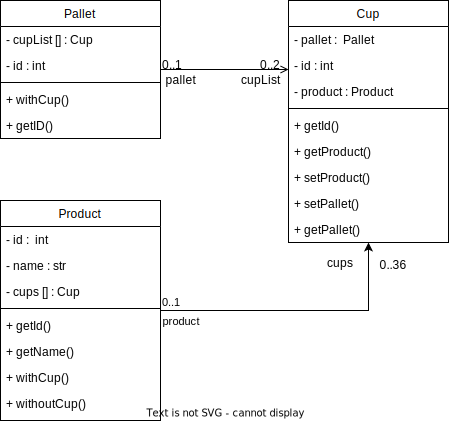
\includegraphics[width = \textwidth ]{Bilder/BeispielRefInt}
        \centering
\end{figure}

In die Klassen der Datenmodelle sollen nur Klassen gespeichert werden, die dynamisch sind. D.h. sie werden zur Laufzeit geändert und/oder
erzeugt bzw. gelöscht. 
Für die Modellierung der Daten wird das MVVC Konzept angewandt und um Serviceklassen erweitert.

Bei der Anlieferung eines Bechers wird dieser in eine Palette gestellt und anschließend eingelagert.
Ein Objektdiagramm dieser Situation ist in Abb.\ref{fig:figure14} dargestellt.

Eine Palette kann keinen, einen oder zwei Becher beinhalten.
Die Becher in einer Liste in dem Paletten-Objekt zu speichern hat den Nachteil, dass man die Becher in der Palette als Listeneinträge verarbeiten muss
und der Slot als weitere Listenspalte geführt wird.

Die Becher als zwei separate Attribute des Paletten-Objekts zu führen hat den Nachteil, dass zwei Orte abgefragt werden müssen.
Andererseits ist die Zuordnung des Bechers zum Slot dadurch inhärent.
Daher wird dieser Ansatz gewählt.

Abb. \ref{fig:figure14} zeigt auch, dass jedes Objekt der Klasse Palette und Cup ein Feld \verb|location| braucht.
Hier wird das Objekt gespeichert in dem sich die Palette oder Becher gerade befindet.

Dies ist erforderlich um referenzielle Integrität zu gewährleisten und erleichtert die Implementierung der Controller,
wie eingangs in Kapitel \ref{PythonApp} beschrieben.

Aus dem Diagramm wird auch deutlich, dass zwsichen den Objekten der Klassen \verb|MobileRobot|, \verb|WorkBench| und
\verb|Inventory| keinerlei Assoziationen gibt.

Es wird also ein weiteres Objekt, z.B. ein InventoryController, gebraucht um aktiv Objekte von einem Lagerort zu einem Anderen
zu schreiben.
Immer wenn ein Service Zugriff auf das Datenmodell braucht, wird der entsprechende Controller diese Zugriffe verarbeiten.
Als Ergebnis dieser Überlegungen leitet sich ein (Daten-)Klassendiagramm ab (Siehe Abb.\ref{fig:figure15}).

\begin{figure}
        \caption[Objektdiagramm]
        {\small Die Abbildung zeigt ein Objektidiagramm aus Ablageorten für Paletten und Becher. Es ist ebenfalls
        ersichtlich, dass keine Verbindungslinien zwischen dem mobilen Roboter, dem Kommissioniertisch und dem Lager existieren.
        }\label{fig:figure14}
        \includegraphics[width = \textwidth ]{Bilder/Objektdiagramm_PaletteCupStorage}
        \centering
\end{figure}

\begin{figure}
        \caption[Klassendiagramm Datenmodell ]
        {\small Klassendiagramm für die Datenstruktur der Software der Lagerverwaltung.
        }\label{fig:figure15}
        \includegraphics[width = \textwidth ]{Bilder/Klassendiagramm_Datenstruktur}
        \centering
\end{figure}

\subsection{Datenklassen}

In den Datenklassen sollen alle realen Objekte abgebildet werden, die durch das Lager bewegt sind oder daran aktiv/passiv beteiligt sind. 
Das betrifft: 

\begin{enumerate}
        \item Becher.
        \item Paletten, weil sie Becher beinhalten können und mit oder ohne Becher bewegt werden. 
        \item Greifer, wei er die Becher und Paletten bewegt. Ein Ausfall der Lagerzelle kann bewirken, dass ein Becher / Palette auf dem Greifer verbleibt.
        \item Kommissioniertisch, weil er Ziel von Transportbewegungen ist.
        \item mobile Roboter, weil er Quelle und Ziel von Transportbewegungen ist.
\end{enumerate}

\subsection{Konstante Daten}

Daten, die über die im Rahmen der Entwicklung festgelegt werden und sich üblicherweise nicht Ändern, sollen in einer
eigenen Klasse gespeichert werden und \verb|constants| heißen. 
Dort soll gespeichert werden: 

\begin{itemize}
        \item Dateipfade zu allen Dateien, die das Programm verwendet oder erzeugt. Dies können z.B. Konfigurationsdateien, Logdateien oder Dateien zum Abspeichern von Daten sein.
        \item Strategische Werte, die in der Entwicklung festgelegt und mehrfach verwendet werden. 
\end{itemize}

\subsection{Programmeinstellungen}

Programm-Einstellungen sollen in einer eigenen Klasse \verb|preferences| gespeichert werden.
Die Einstellungen sollen in einer Datei gespeichert werden, sobald der Benutzer eine Änderung speichert.

\section{Konzepte für Controller- und Serviceklassen}\label{ControllerServices}

Die Kommunikation über Modbus wird durch OPC UA ersetzt.
Für die Kommunikation über diese Schnittstelle wird ein \verb|OpcUaService| implementiert.

Ein Service übernimmt die Kommunikation mit den RFID-Lesegeräten in der $\mu$Plant und stellt die ausgelesenen Daten
über den \verb|OpcUaService| den anderen Stationen zur Verfügung.

Das in \cite{LarsKistner2017} eingeführte Agentensystem wird ebenfalls als eigener Service implementiert.
Da die LZ nicht mit anderen Stationen kommunizieren muss, reicht die Implementierung des Clients.
Dabei wird die Kommunikation über OPC UA realisiert.

Controller werden gebraucht um Schnittstellen zwischen Service und Daten oder zwischen Service und GUI zu implementieren.
Eine besondere Rolle nimmt der \verb|InventoryController| ein.

Er muss zum Start des Programms das Inventar aus Dateien laden und damit das Datenmodell initialisieren.
Aus Gründen die in Kapitel \ref{Fehlerbehandlung} erörtert werden, sollte der Controller nach jeder vollständigen Änderung
des Datenmodells die Änderung einerseits in der Datei sichern.

Eine Liste aller benötigter Service Klassen ist in Tab. \ref{tab:Services} aufgelistet.
Die Controller finden sich in Tab. \ref{tab:Controller}.


\begin{table}[h]
\centering
\caption{Benötigte Serviceklassen}
\begin{tabularx}{\textwidth}{|l|X|}
\hline
Klassenname & Beschreibung \\
\hline
Modbus Service & Implementiert die Modbus Kommuniktaion, sendet Modbus informationen an entsprechende Controller\\
\hline
OPC UA Service & Hält OPC UA Server und Client, organisiert Kommunikation zu anderen OPC UA entities\\
\hline
RFID Service & Erledigt alles was mit RFID zu tun hat\\
\hline
\end{tabularx}\label{tab:Services}
\end{table}


\begin{table}[h]
\centering
\caption{Werte der Klasse ModbusBaseAddress}
\begin{tabular}{|l|l|}
\hline
Klassenname & Beschreibung \\
\hline
InventoryController & Führt jede Operation bezüglich des Datenmodells aus \\
\hline
EventlogController & Erzeugt Meldungen für den Eventlog\\
\hline

\hline
\end{tabular}\label{tab:Controller}
\end{table}



\section{GUI Konzeptionierung}

Neben der Datenmodellierung und der Programmlogik ist die GUI ein wichtiger Bestandteil der Software.

\subsection{PySide6 und QuickQml 2.0}

Laut der Qt Wiki Website \cite{QtWikiHistory} wurde das Qt Framework geboren, als ihre Schöpfer Haavard Nord und
Eric Chambe-Eng im Sommer 1990 in Norwegen an einem GUI für eine Ultraschalldatenbank arbeiteten.

Die Software sollte damals in C++ implementiert auf Mac, Unix und Windows laufen.
Fünf Jahre später veröffentlichten Sie das erste Qt Framework unter dem Firmennamen Troll Tech.
Seitdem gewann das Framework immer mehr Popularität.
Im Jahr 2006 übernahm Nokia die Firma Troll Tech und verkaufte das Qt Project in den Jahren 2011 und 2012 erst teilweise,
dann vollständig an den Digia Konzern.
Seit 2014 ist Qt als Tochterunternehmen des Digia Konzerns unter dem Namen \glqq The Qt Company\grqq{} ein eigenständiges Unternehmen.

Das Qt Framework ist in C++ implementiert.
Die neue Software für die $\mu$Plant soll jedoch in Python implementiert werden.
Für diese Zwecke hat Qt u.A. das Framework PySide6 veröffentlicht, welches einen Wrapper für Python Projekte bietet.

GUI's können in PySide6 zwei Paradigmen folgend erstellt werden.

Eine Möglichkeit ist es, das GUI über Widgets\cite{pysideQtWidgets} zu erstellen.
Dabei werden GUI Elemente als eigene Klasse direkt im Python implementiert.
Dies ist eine schnelle und unkomplizierte Art einfache GUIs zu erstellen. 

Die zweite Möglichkeit ist QtQuick \cite{pysideQtQuick} zu nutzen. 
Neben der Instanz einer \verb|QGuiApplication| wird eine \verb|QQmlApplicationEngine| instanziiert.
GUI Elemente werden in einer separaten QML-Datei erstellt und mit dieser geladen und gerendert. 
Dies bietet den Vorteil, dass für das GUI eine deklarative Sprache verwendet wird, die sich von der Programmlogik trennt.
Die Bibliothek \verb|QtQuick 2.0| beinhaltet viele grundlegende QML-Datentypen, die beliebig zu GUIs kombiniert werden können.

Für die Umsetzung eines MVVC-Design Patterns empfiehlt sich die Verwendung von QML.
Durch die Verwendung des Frameworks wird die konsequente Trennung zwischen Interface und Datenmodell erzwungen.
Veranschaulicht wird dies in Abb. \ref{fig:figure10}.


Um die anwendungsspezifischen Datenmodelle (Model) in einem GUI (View) zu verwenden, muss das Datenmodell als Ressource
der \verb|QQmlApplicationEngine| zur Verfügung gestellt werden.
Zu diesem Zweck werden Klassen implementiert, die von Qt-Klassen erben, die wiederumg von \verb|QtAbstractModel| abgeleitet sind.
Die Klasse muss der Datenstruktur des Datenmodells entsprechen. In diesem Projekt sind \verb|QAbstractListModel| für Listen
und \verb|QAbstractTableModel| für tabellenartige Datenstrukturen relevant.

In diesen Klassen müssen bestimmte Methoden überschrieben werden. Manche andere Methoden sind optional. 
Welche Methoden das sind ist in der Referenzdokumentation des Qt Frameworks nachzulesen.

Die Implementierungen der Methoden ist individuell und hängt von der Datenstruktur ab. Die Datentypen der Argumente und Rückgabewerte sind 
jedoch vorgegeben.

Wenn in einem GUI z.B. eine Liste sortiert oder gefiltert werden soll, dann muss zusätzlich ein sog. \verb|QSortFilterProxyModel|
implementiert werden. 

Bevor die Instanz der \verb|QQmlApplicationEngine| die erste QML-Datei lädt - also vor Programmstart - muss entweder die Instanz des
\verb|QSortFilterProxyModel| oder die Instanz des \verb|QAbstractModel| als Ressource der \verb|QQmlApplicationEngine| registriert werden.
Diese Instanz ist dann das Viewmodel. Die Implementierten Methoden dienen dazu die Daten des Datenmodells beim Rendern zu verarbeiten. 

Über das GUI können die Daten des Viewmodels geändert, gelöscht oder hinzugefügt werden - ohne zwangsweise das Datenmodell selbst zu ändern.

Wenn ein Viewmodel mit der \verb|QQmlApplicationEngine| verknüpft ist, kann es über seine URI in jeder QML-Datei angesprochen werden.

In einer QML-Datei wird einem entsprechenden QML-Datentyp, z.B. \verb|ListView| für eine einfache Liste,
über das Property \verb|model| die URI des Datenmodells zugewiesen.
Dadurch kennt das \verb|ListView| Objekt die Indices des Datenmodells und erhält beim Rendern der Liste nur die benötigten
Daten.

Jede weitere Aktion, die durch den Benutzer auf ein Listenelement ausgelöst wird, bezieht sich auf ein Delegate des Datenmodells.
Jede Änderung an dem Delegate wird zunächst gerendert und überprüft bevor das Datenmodell geändert wird.
Diese Basisfunktion kommt mit dem Qt Framework an sich und muss nicht implementiert werden.
Wie jedoch das Datenmodell mit den geänderten Daten umgeht oder ob die Änderung des Datenmodells automatisch ein Update
der Daten auf dem Server oder der Datei auslöst, muss vom Entwickler implementiert werden!

Die Kommunikation des GUIs mit der Anwendung erfolgt über Signale und Slots.
Signale sind Teil des Signal/Slot Prinzips des Qt Framework \cite{pysideSignalSlot} und stellen die Funktion eines Events dar.
Wird ein Signal an beliebiger Stelle im GUI emittiert, kann es an jeder anderen Stelle als Event genutzt werden.
Dadurch muss man in der Regel keine zusätzlichen Callbacks oder Lamda-Ausdrücke benutzen.

Außerhalb des QML-Contexts, z.B. in einer Python Klasse, muss das Signal der Klasse bekannt sein, indem das Signal an die Klasse
gebunden wird.

Eine Funktion, die mit der Annotation \glqq @Slot()\grqq{} versehen ist, wird als Slot behandelt und kann mit dem Signal
verknüpft werden, sodass diese bei Auftreten des Signals ausgeführt werden.

Ist eine Methode einer Klasse ein Slot und ist diese Klasse als Ressource der \\\verb|QQmlApplicationEngine| registriert,
dann kann im QML-Code der Slot der Klasse auch direkt aufgerufen werden. 

An Signale und Slots können Daten übergeben werden.
Bei der Deklaration eines Signals oder Slots müssen als Argumente für jedes übergebene Datum der Datentyp angegeben werden. 
z.B.: $$@Slot(str, int)$$

Anzahl und Datentyp der Argumente müssen bei deklarierten Signalen und Slots jederzeit übereinstimmen. 
Dass Datentypen in Python dynamisch sind kann unter Umständen zum Problem werden. 
Der Datentyp \verb|None| ist im QML-Kontext nicht bekannt und führt zu einer Fehlermeldung. 
Es kann also erforderlich sein die zu übergebenen Daten auf die Datentypen zu casten oder in sinnvolle Werte umzuwandeln.

In meiner Vorbereitung auf diese Arbeit hat sich eine intuitive Vorgehensweise entwickelt, die ich für die Implementierung
der Software empfehlen möchte:

Beim Initialisieren des Programms werden alle Datenmodelle (\verb|QAbstractModel| und abgeleitete Klassen), Controller
und Serviceklassen instanziiert und als Root-context der \verb|QQmlApllicationEngine| gesetzt.
Siehe dazu das Beispiel \ref{exampleApp}.
Damit stehen sie dem Programmierer in jeder QML-Datei der Anwendung zur verfügung.

In einer QML-Datei können die Kontexte der QQmlEngine nun unter ihrer URI referenziert werden.
Dies ist in Beispiel \ref{exampleListview} gezeigt:

In dem QML-Datentyp \glqq ListView\grqq{} wird dem Property \verb|model| die URI des ListModels aus \ref{exampleApp} zugewiesen.
Im weiteren Verlauf des Codes findet sich ein \verb|MouseArea| QML-Datentyp.

Wird in dem Bereich ein Klick mit linker Maustaste durchgeführt, wird das Signal \\\verb|onClicked| emittiert.
Innerhalb des Codes im Funktionskörper der \verb|MouseArea| ist definiert, dass nach einem Mausklick die Funktion \verb|selectRow(message)|
aufgerufen wird. \verb|message| ist dabei der übergebene Parameter.

Das Beispiel braucht dabei keinerlei Importe anderer Klassen, was daran liegt, dass sowohl das DatenModell als
auch das Objekt der Controller Klasse als Ressource der QQmlEngine registriert wurden.

Im weiteren Verlauf des Codes wird ein QML-Datentyp \verb|Connections| dazu benutzt, das Signal des Controllers \verb|onRowClicked|
mit einer Funktion zu verbinden.
Die Funktion wird innerhalb des \verb|Connections|-Datentyps in JavaScript implementiert.

Gemäß der Namenskonvention ist das Signal im Controller selbst als \verb|RowClicked| deklariert!
Innerhalb der QML-Datei werden die Signale dann mit dem Präfix \glqq on\grqq{} erfasst.

Der Signalname wird als Name einer JavaScript-Funktion verwendet, die mit \verb|function| gekennzeichnet ist.
Der Code innerhalb des Funktionskörpers beschreibt dann die Funktionslogik im JavaScript-Syntax.
Im Fall des Beispiels wird ein bool'sches Property umgeschaltet, wenn die \verb|id| des Datenmodell-Delegates mit der
\verb|message| des Signals übereinstimmt.

\lstset{
    basicstyle=\small\ttfamily
}
\newpage
\lstinputlisting[language=Python,
        caption ={Beispiel einer einfachen App mittels PySide6. \small Zunächst wird eine Instanz der
Application-Klasse und der QmlEngine erzeugt. Danach werden Objekte eines Datenmodells und
eines Controllers erzeugt und als rootContext der QmlEngine registriert. Anschließend wird die QML-Datei des Hauptfensters geladen,
was die App startet.}]
{Listings/Demo1.py}\label{exampleApp}

\lstinputlisting[language=xml,
caption ={Beispiel einer QML-Datei\small Diese QML-Datei erzeugt ListView QML-Datentyp, der zum Anzeigen der Daten
in einem ListModel verwendet wird. Innerhalb eines Rechtecks mit farbigem Rand werden in einem RowLayout Type die
Datensätze des Datenmodells gerendert und über die Funktionslogik von Signalen der QML-Datentyps und der Controllerklasse
farblioch markiert.}]{Listings/listviewExample.qml}\label{exampleListview}
\newpage

\begin{figure}
        \caption[Model-View Konzept mit zusätzlichem Controller und Service ]
        {\small Die Abbildung zeigt das in PySide6 verwendete Model-View Konzept, welches um einer Controllerklasse und
        einer Service Klasse erweitert wurde. }\label{fig:figure10}
        \includegraphics[width = \textwidth ]{Bilder/MVCS_Beispiel}
        \centering
\end{figure}

\newpage

Aus den Beispielen \ref{exampleApp} und \ref{exampleListview} lässt sich eine Systematik erkennen:
Die Daten sind hinter einem ViewModel geschützt und werden der View zur Verfügung gestellt.

Über die QML-Dateien erfolgt die GUI Modellierung und Events werden mit dem Signal/Slot Prinzip behandelt.
Beliebige Ressourcen können als Teil der QmlEngine registriert werden, um Sie an anderer Stelle verfügbar zu machen.

Das künftige Programm soll jedoch auch Programmteile aufweisen, die nicht unbedingt mit den Daten oder dem GUI verknüpft sind.

Z.B. die Kommunikation über ModBus und zum ABB Industrieroboter oder das Übersetzen der Modbus Werte in
RAPID Befehle.
Diese Programmteile werden als Service Klassen bezeichnet.
Wenn sich der Programmcode auf ein GUI auswirkt, wird ein Controller gebraucht, der dieses Verhalten steuert.

Die Funktionen eines Services in den Controller zu integrieren würde die Wartbarkeit und Erweiterbarkeit verschlechtern.

Nach der Systematik wie in Abb. \ref{fig:figure10} abgebildet, können beliebig viele Datenmodelle, GUI's, Controller und Services
parallel existieren ohne sich gegenseitig zu beeinflussen.

Als Nachteil kann angeführt werden, dass sich mit zunehmendem Kontextregister der QmlEngine die Performance des Programms
verschlechtern wird.
Bei dem eher gering erwarteten Funktionsumfang der zu erstellenden Software wird dies jedoch untergeordnet behandelt und könnte
durch das Aufteilen der Funktionen in Threads reduziert werden.

\section{GUI - Modellierung}

Die Hauptfunktion der Software ist das automatisierte Abarbeiten der Kommissionsaufträge, die bisher über Modbus TCP/IP
von der Auftragsverwaltung der $\mu$Plant übergeben werden.
Während der Automatikbetrieb läuft, wird ein Benutzer allenfalls einen Soll-Ist-Vergleich zwischen dem Stand der 
Software und der realen Lagerzelle durchführen.
Die Idee ist daher, dass das neue GUI im Vergleich zum Alten aufgeräumter und übersichtlicher wird. 
Informationen die unmittelbar mit dem Prozess verbunden sind, sollen leicht ersichtlich und verfügbar sein. 
Alle anderen Informationen sollen nur bei Bedarf angezeigt werden.

In Abb. \ref{fig:figure11} zeigt meinen Entwurf zu dieser Idee:

Links ist die Andockstation des mobilen Roboters simuliert mit einem RFID Gerät darüber.
Die eingelesen Daten des RFID -Lesers könnten rechts daneben angezeigt werden, sobald der Benutzer mit der Maus 
darüber hovert. Wenn aktuell ein Tag gelesen wird, könnte das Symbol die Farbe wechseln.

Der Kommissioniertisch ist mit seinen beiden Plätzen \glqq K1\grqq{} und \glqq K2\grqq{}  daneben symbolisiert.

Die Visualisierung des Lagers nimmt die gesamte rechte Bildschirmhälfte ein.

Die Produktliste, wie sie in \ref{fig:figure} Bereich \glqq D\grqq{} dargestellt ist, ist im GUI nicht mehr vorhanden.
Muss der Bediener ein Produkt an irgendeiner Stelle des Programms überschreiben, so wird ihm nicht mehr die Produkt-ID
angezeigt, sondern direkt der Produktname.
Zusätzlich kann die Produktliste als Neues Fenster über die Toolbar eingeblendet werden.

Sämtliche Einstellungen wie IP und Port der Kommunikationsschnittstellen werden nur selten gebraucht.
Über die Toolbar sind die Einstellungen über den QML-Datentyp \verb|QDialog| einsehbar.

Eingegebene Daten müssen bestätigt werden und können auch wieder verworfen werden.

Die Bereiche \glqq E\grqq{} (Inventarliste) und \glqq F\grqq{} (Eventlog) aus Abb. \ref{fig:figure} müssen nicht
gleichzeitig sichtbar sein. 
Sie werden in einem Register integriert und mit dem QML-Datentyp \verb|StackView| oder einem Loader angezeigt.
Das Erscheinungsbild der beiden GUI Elemente kann aus der alten Software übernommen werden.
Als Drittes Register soll zusätzlich zum alten Startbildschirm eine Commission List (siehe Abb. \ref{fig:figure13}) hinzugefügt werden.
Sie soll eine Übersicht über die von der Auftragsverwaltung eingetroffenen Aufträge und ihren Status anzeigen.

Um manuelle Überschreibungen der Produkte und Becher vorzunehmen, wird statt des Checkbox-Menüs ein Zahnrad-Symbol erscheinen,
wenn man über dem entsprechenden Bereich den Mauszeiger führt (Hovering).
Mit Klick auf das Zahnrad-Symbol soll ein Objekt des QML-Datentyps \verb|QDialog| eingeblendet werden in dem die alten
Feldwerte angezeigt und editiert werden können, aber auch das Editieren verworfen werden kann.


Die Funktion des ehemaligen Controllers wird über die Toolbar aufgerufen.
Der Begriff \glqq Controller\grqq{} an sich ist im Zusammenhang mit der neu konzipierten Software irreführend und wird daher verworfen.
Der stattdessen wird der Titel \glqq Manual Processing\grqq{} gewählt.
Hiermit sollen manuell Transportaufträge erzeugt werden wie z.B. \glqq Räume den Becher aus Lagerort L3a nach L6b\grqq{}.
Dies soll für jede sinnvolle Transportoperation möglich sein.
Mit Klick auf den entsprechenden Eintrag in der Toolbar öffnet sich ein Fenster oder ein Dialog, wie in Abb.\ref{fig:figure12}.
Die so neu erzeugten Transportaufträge werden ebenfalls in der Commission List (siehe Abb. \ref{fig:figure13}) angezeigt.


\begin{figure}
        \caption[Mockup des Startbildschirms]
        {\small Die Abbildung zeigt wie der Startbildschirm aussehen könnte um die Funktion des Automatikbetriebs abzubilden:
        }\label{fig:figure11}
        \includegraphics[width = \textwidth ]{Bilder/Mockup_Startbildschirm}
        \centering
\end{figure}

\begin{figure}
        \caption[Mockup des Menüs für die manuelle Lagersteuerung]
        {\small Die Abbildung zeigt, dass entweder ein Becher oder eine Palette (mit oder ohne Becher) vom Startort zum
        Zielort transportiert werden kann. Die Eingabe der Zielorte wird hier über zwei Dropdown Menüs realisiert.
        Das Mockup impliziert, dass bei Tätigung einer Eingabe eine Validierung der Eingaben erfolgt.
        }\label{fig:figure12}
        \includegraphics[height = 0.5\textwidth ]{Bilder/Mockup_ManualProcessing}
        \centering
\end{figure}

\begin{figure}
        \caption[Mockup der Commission List]
        {\small Die Abbildung zeigt, wie die Commission List aussehen könnte. Sie könnte als Tab in einem Register eingebunden werden.:
        }\label{fig:figure13}
        \includegraphics[width = \textwidth ]{Bilder/Mockup_CommissionList}
        \centering
\end{figure}
\vspace{1cm}

Das GUI des RFID Server Programms war sinnvoll und praktisch und kann so wie bisher umgesetzt werden.
Der Aufruf des Programms soll über die Toolbar implementiert werden.

\newpage
\section{Teilautomatisierte Code Dokumentation mit Sphinx}

Code-Dokumentation ist ein wichtiger Bestandteil jedes Softwareprojekts und dient dazu den Code anderen Entwicklern zugänglich zu machen.
Die Erstellung ist unter Umständen aufwändig, kann aber zumindest teilweise automatisiert werden.
Eine Möglichkeit besteht darin, das Paket sphinx zu verwenden.

Sphinx ist ein Tool, das es Entwicklern ermöglicht, Dokumentationen in verschiedenen Formaten wie HTML, PDF und ePub
aus Kommentaren im Code des Python Projekts zu erstellen.
Dazu werden die in Python üblich Docstrings verwendet \cite{pepDocstrings}.

Das Paket kann über PyPi mit folgendem Kommando über die Eingabeaufforderung installiert werden:
\begin{lstlisting}
        pip install -U sphinx
\end{lstlisting}


Das Sphinx- Paket benutzt Themes um die Dokumentation grafisch darzustellen und zu strukturieren.
In Vorbereitung auf diese Arbeit habe ich mir das rtd-theme (Read the Docs \cite{RTD}) angeschaut und ausprobiert.
Es ist ein beliebtes Theme für Sphinx-Dokumentationen, da eine klare und übersichtliche Darstellung der Dokumentation
bietet und einfach zu verwenden ist.
Um das rtd-theme in einem Sphinx-Projekt zu verwenden, muss es zunächst installiert werden.
Dies kann über den Befehl
\begin{lstlisting}
        pip install sphinx_rtd_theme
\end{lstlisting}
erfolgen, dabei wird das Sphinx Paket auf die Version 6.4.1 angepasst.

Um Sphinx zu nutzen, muss es zunächst konfiguriert werden. Mit dem Kommando

\begin{lstlisting}[language = python]
        sphinx-quickstart
\end{lstlisting}
wird man Über die Konsole aufgefordert einige Optionen festzulegen mit denen die Dokumentation aufgesetzt wird.
Anschließend befinden sich in dem ausgewählten Ordner:
\begin{itemize}
        \item ein Makefile
        \item eine Datei \verb|modules.rst|
        \item eine Datei \verb|index.rst|
        \item eine Datei \verb|conf.py|
\end{itemize}

Die Index-Datei ist später der Einstiegspunkt.
Im RST-Format \cite{sphinxRST}kann die Seite gestaltet werden.

In der \verb|modules.rst| dagegen werden die Module aufgelistet, die dokumentiert werden sollen.
Nach der Installation des rtd-theme kann es in der Konfigurationsdatei von Sphinx aktiviert werden.
Dazu muss die Zeile \verb|html_theme = 'sphinx_rtd_theme'| in die Datei \verb|conf.py| eingefügt werden.
Sobald das Theme aktiviert ist, wird die Dokumentation nach dem build Vorgang im rtd-Theme angezeigt.

\subsection{Sphinx Erweiterungen}\label{subsec:sphinx-erweiterungen}

Erweiterungen werden nach der Installation des Pakets in der Konfigurationsdatei \verb|conf.py| aktiviert.
Im Rahmen habe ich viele Erweiterungen getestet und empfehle die nachfolgenden Erweiterungen zu verwenden. 
Die nachfolgende Zeile aktiviert alle Erweiterungen aus meiner Empfehlung. 

\begin{lstlisting}[language = python,label={lst:sphinxExt}]
extensions = [
        'sphinx.ext.autodoc',
        'sphinx.ext.viewcode',
        'sphinx_copybutton']
\end{lstlisting}

\subsubsection{Autodoc}

Autodoc wird dazu verwendet um die Docstrings im Python-Code als Dokumentationstext zu erfassen.
Damit dies funktioniert muss ein Modul in der Datei \verb|modules.rst| mit folgendem Syntax hinzugefügt werden:

\begin{lstlisting}[language = python,label={lst:sphinxAutomodule}]
.. automodule:: src.cameraApplication.cameraProcessing
        :members:
        :undoc-members:
        :show-inheritance:
\end{lstlisting}

\verb|:members:| sorgt dafür, dass alle Klassen und Funktionen des Moduls in der Dokumentation erscheinen.
Die verwendeten Docstrings wirden zusammen mit dem Namen und ggf. Argumenten und Rückgabewerten angezeigt.

\verb|:undoc-members:| sorgt dafür, dass auch Funktionen und Klassen ohne Docstrings in der Dokumentation erscheinen.
Die Klassen und Funktionen werden dann ohne Beschreibung angezeigt.

\verb|:show-inheritance:| sorgt dafür, dass die Vererbungshierarchie der Klassen angezeigt wird.
Dies ist in Verbindung mit dem Qt Framework oft hilfreich. Da viele Qt-Klassen eine große Vererbungskette haben, kann dies manchmal auch unübersichtlich werden.

Die Dateipfade der Module werden wie im Beispiel vom Makefile aus zur Python-Datei angegeben, jedoch ohne Dateierweiterung.
Docstrings in den Modulen werden direkt als HTML gerendert.
Inline-Kommentare werde nicht angezeigt.

QML-Dateien können auf diese Weise nicht gerendert werden. Um sie dennoch in der Dokumentation anzuzeigen,
habe ich sie in der Datei \verb|modules.rst| mit folgendem Syntax hinzugefügt:

\begin{lstlisting}[language = python,label={lst:sphinxQML}]
        qml.main.qml
        ------------
        
        The main QML-file creates the main application window.
        
        .. literalinclude:: src/qml/main.qml
                :language: qml
        \end{lstlisting}
Dadurch wird der gesamte Inhalt der QML Datei in der Dokumentation angezeigt.

\subsubsection{viewcode}

Um den Quellcode des Moduls in dem HTML Dokument einblenden zu können wird die Erweiterung viewcode genutzt.
Unterhalb der Modulüberschrift im HTML-Dokumentwerden zunächst alle Docstrings gerendert.
Darunter erscheint nun ein grauer Bereich, in dem Python Code mit Farbformatierung angezeigt wird.
Es werden auch andere Sprachen erkannt, jedoch gibt es leider keine Option QML Code farblich formatiert
anzuzeigen.
QML-Dateien werden im Allgemeinen von Autodoc nicht erkannt.
Die Einzige Option ist ein \verb|literalinclude| Befehl wie oben schon beschrieben.
Wie leicht zu erkennen werden Docstrings nicht erkannt und müssen daher manuell eingefügt werden.
Kommentare im JavaScript-Syntax und Properties werden farblich hervorgehoben.

\subsubsection{sphinx\_copybutton}

Diese Erweiterung fügt in Code-Blöcken der HTML-seite eine Kopier-Taste hinzu, mit denen 
z.B. Kommandozeilenbefehle in den Zwischenspeicher kopiert werden können.
Code-Blocks werden wie folgt angegeben:
\begin{lstlisting}[label={lst:sphinxCodebutton}]
        .. code-block:: bash
                pip install -r requirements.txt
\end{lstlisting}


\section{Sonstige Festlegungen}

Die zu verwendenden Farben sollen dem $mu$Plant Logo oder dem Logo der Universität Kassel entnommen werden.

\subsection{Virtual Environment}

Die Entwicklung der Software soll mit einer virtuellen Entwicklungsumgebung (venv) stattfinden.
Alle benötigten Pakete werden dort installiert.

Die installierten Pakete werden nicht in das Git Repository gepusht. Stattdessen wird mit
\begin{lstlisting}[label={lst:freezeReq}]
        pip freeze > requirements.txt
\end{lstlisting}
Eine Textdatei mit allen verwendeten Bibliotheken erstellt.
Läd sich ein Benutzer das Repository herunter, können mit dem Befehl
\begin{lstlisting}[label={lst:installReq}]
        pip install -r requirements.txt
\end{lstlisting}
alle benötigten Pakete installiert werden, sodass das Projekt lauffähig kompiliert werden kann.
Der Nachteil ist, dass es im Aufgabenbereich des Entwicklers liegt, nicht verwendete Pakete zu deinstallieren,
sodass sie später nicht unbeabsichtigter Weise installiert werden.


\subsection{Verwendete Programme }

Nachfolgend werden alle verwendeten Programme und Software aufgelistet, die zur Erstellung der Software benutzt werden
\begin{itemize}
        \item PyCharm Comunity Edition von JetBrains wird zur Editierung von Code verwendet. Das betrifft nicht nur Python Code,
        sondern auch alle anderen Sprachen und Syntaxe exklusiv QML. Sogar zur Erstellung von LaTeX Dokumenten wird
        PyCharm mit dem PlugIn TeXiFy verwendet.
        \item Qt Creator kann für alle Qt kompatiblen Programmiersprachen verwendet werden. Es beinhaltet außerdem den
        Qt Designer, mit dem QML-Dateien grafisch editiert werden können. Das Programm ist teilweise unbequem und umständlich,
        ist aber für QML in Python die beste Lösung um intuitiv Einstellungen an QML-Datentyps auszuprobieren.
        \item Visual Studio 2022 wird dazu verwendet den C\# Code der alten Software zu analysieren.
        Das PlugIn \glqq Class Designer\grqq{} wird dazu verwendet um die Projektmappen in Klassendiagramme darzustellen.
        \item Die Homepage Diagrams.net bietet eine gute Lösung um schnell Diagramme in UML und anderen Standards zu erstellen und
        in gewünschten Dateiformaten zu exportieren.
        \item Pictogramme und Symbole werden mit Adobe Illustrator erstellt.
\end{itemize}
\cleardoublepage

\chapter{Analyse zur Fehlerbehandlung}\label{Fehlerbehandlung}

\subsection{Fehleridentifikation}

Fehler können systematischer oder sporadischer Natur sein.
Systematische Fehler können in der Softwareentwicklung durch intensives Testen behoben werden.
In Python ist dies beispielsweise mit dem Paket \verb|pytest| ( siehe \cite{pytestHP}) oder \verb|unittest| ( siehe \cite{unittestHP}) möglich.
Anhand einer kurzen Recherche beider Internetauftritte werde ich pytest verwende.
Einerseits liefert pytest bei fehlgeschlagenen Tests eine ausführlichere Analysemeldung, adererseits wird pytest von Qt empfohlen.
Mit pytest lassen sich aber nur Python Module testen.
Für einen GUI Test muss das \verb|QtTest| Framework verwendet werden.
Leider lässt sich zu diesem Paket keine umfangreiche Dokumentation, sodass von diesem Framework in dieser Arbeit abgesehen wird.\\

\vspace{1cm}
Sporadische Fehler können nicht vorhergesehen werden und müssen überprüft und abgefangen werden.
Die erwarteten Quellen sind Eingabefehler und Kommunikationsfehler.

\subsection{Erkennung fehlerhafter Benutzereingaben}

Werden im Programm falsche Daten eingegeben, soll dies, soweit wie möglich, überprüft und abgefangen werden.
Die Tabelle \ref{tab:Benutzereingaben} listet alle erwarteten Benutzereingaben und mögliche Methoden die Benutzereingaben
zu validieren. \\

\begin{table}[h]
\centering
\caption{Benutzerinageben, mögliche Fehler und ihre Erkennung}
\begin{tabularx}{\textwidth}{|l|p{2cm}|p{2cm}|X|}
\hline
Art & Typ & Wertebereich & Fehlererkennung \\
\hline
IP Adresse & Formatierter String aus Integers & 0 \ldots 255 bzw. 0 \ldots 9 & Gültigkeitsprüfung bei Dateneingabe, Validierung bei Verbindungsaufbau\\
\hline
IP Port & Integer & 0\ldots65536 & Wertebereich bei Dateneingabe, Validierung bei Verbindungsaufbau\\
\hline
Produkt ID & Integer & 0\ldots99 & Eingabe anhand Dropdown Menü mit Anzeige des Produktnamens beschränkt Wertebereich auf zulässige Werte. Validierung nur im Softwarebetrieb durch Soll-Ist Abgleich.\\
\hline
Becher ID & Integer & 0\ldots99 & Eingabe kann nicht auf gültigen Wertebereich beschränkt werden. Soll-Ist-Vergleich mittels RFID ist möglich.\\
\hline
Palette & Bool & True / False & Abgleich mit Anwesenheit von Bechern, arUco Marker Erkennung mittels Kamera\\
\hline
\end{tabularx}\label{tab:Benutzereingaben}
\end{table}



\vspace{1cm}
Wenn manuell Transportaufträge eingegeben werden, kann es zu Konflikten kommen.
Z.B. Könnte im Abholort kein Becher oder keine Palette sein.
Umgekehrt könnte am Abstellort eine Palette oder Becher stehen.
Für diese Problematiken können :
\begin{itemize}
    \item Inventardaten zur Überprüfung herangezogen werden
    \item Kameragestützte Validierungsprozesse in Kapitel \ref{Kap5} Entworfen werden.
\end{itemize}
\cleardoublepage

\chapter{Ideensammlung zu kameragestützten Validierungsprozessen in der Lagerverwaltung}\label{Kap5}

    \subsection {Konzepte}

    \subsection {Abgeleitete Anforderungen an die Kamera}

    \subsection {Kameraauswahl}
\cleardoublepage

% !TeX spellcheck = de_DE
\chapter{Zusammenfassung und Ausblick}

In dieser Arbeit wurde ein breiter Themenbogen gespannt, der von der Analyse der Architektur und Funktion einer C$\#$ / .NET Softwareanwendung bis zur
Konzeptionierung einer neuen Anwendung in Python mit Qt reicht.
In der Auseinandersetzung der Programmiersprachen C$\#$ und Python wurden ihre Unterschiede diskutiert und aufgezeigt, dass eine Portierung 1:1 nicht möglich ist.
Eher handelt es sich dabei um eine Neuentwicklung, die die Funktionen der alten Software übernimmt und um den neuen Kommunikationsstandard OPC UA erweitert.

Mit Augenmerk auf das GUI, wurden wesentliche Informationen und ihre Visualisierung diskutiert und Entwürfe für die neue Anwendung vorgestellt. 
Eine Analyse hat gezeigt, dass der Hauptbildschirm aufgeräumt werden kann, sodass der Hauptbildschirms den Lagerprozess und die Lager-Visualisierung
fokussiert. 
Diejenigen Informationen, die dabei nicht mehr angezeigt werden, können dabei in einem Dialog oder einem neuen Fenster angezeigt werden.
Der Dienst zur manuellen Lagerbedienung wird, genau wie der RFID-Server, als Plugin ausgeführt.

Aspekte der Implementierung wurden diskutiert und veranschaulicht, wie der Aufbau der neuen Anwendung unter Berücksichtigung des MVVC-Konzepts gelingen kann. 
Es wurde detailliert auf die Datenmodellierung eingegangen und die Vorteile der Referenziellen Integrität diskutiert und an Beispielen gezeigt.

Für die Zukunft wurde festgelegt, dass die Weiterentwicklung und Wartung der Anwendung bereits bei der Entwicklung der neuen Anwendung berücksichtigt werden soll. 
Zu dem Zweck werden die einzelnen Controller- und Serviceklassen auf eine enge Kernfunktion beschränkt. 
Die Verwendung der in Python eingebetteten Doc-Strings soll verwendet werden, um mit dem Paket Sphinx eine automatisierte Dokumentation zu erstellen.
Es wurden zudem zwei andere Pakete vorgestellt und diskutiert, mit denen Python-Module getestet werden können, um schnell die Konsistenz des Datenmodells zu überprüfen.
Diese beiden Aspekte sollen es anderen Personen erheblich erleichtern sich in die neue Anwendung einzuarbeiten, um sie zu warten oder zu erweitern.

Der Schwerpunkt des Ausblicks liegt auf der Ideensammlung für kameragestützte Validierungsprozesse in der Lagerzelle.
Es wurden zwei Usecases vorgestellt und Aspekte des Ablaufs diskutiert.
Aus den Ideen wurden Anforderungen an die Kameras und die Implementierung der Software abgeleitet.

%%% Local Variables:
%%% mode: latex
%%% TeX-master: "../MRT-Bericht2020"
%%% End:

\cleardoublepage

% --------------------------------------------------------------------------
% Anhang (WENN NÖTIG)
% --------------------------------------------------------------------------
\appendix
%\pagenumbering{roman}\setcounter{page}{1}
\pagenumbering{Roman}\setcounter{page}{\value{SeitenzahlSpeicher}}

% !TeX spellcheck = de_DE

\chapter{Dies ist der erste Anhang}

Hier Text einfügen.

\cleardoublepage

% --------------------------------------------------------------------------
% Literatur (IMMER)
% --------------------------------------------------------------------------
\addcontentsline{toc}{chapter}{Literaturverzeichnis}

%\bibliographystyle{Literatur/IEEEtran}
%\bibliographystyle{Literatur/IEEEtranS}
%%Deutsch (Groß/kleinschreibung)
\bibliographystyle{Literatur/IEEEtranGER}
%%Deutsch (Groß/kleinschreibung) + DOI
%\bibliographystyle{Literatur/IEEEtranGERdoi}
\bibliography{Literatur/Semesterarbeit}
	
% --------------------------------------------------------------------------
% Ende des Dokuments
% --------------------------------------------------------------------------
\end{document}

%%% Local Variables:
%%% mode: latex
%%% TeX-master: t
%%% End:
